\documentclass[]{article}
\usepackage{lmodern}
\usepackage{amssymb,amsmath}
\usepackage{ifxetex,ifluatex}
\usepackage{fixltx2e} % provides \textsubscript
\ifnum 0\ifxetex 1\fi\ifluatex 1\fi=0 % if pdftex
  \usepackage[T1]{fontenc}
  \usepackage[utf8]{inputenc}
\else % if luatex or xelatex
  \ifxetex
    \usepackage{mathspec}
  \else
    \usepackage{fontspec}
  \fi
  \defaultfontfeatures{Ligatures=TeX,Scale=MatchLowercase}
\fi
% use upquote if available, for straight quotes in verbatim environments
\IfFileExists{upquote.sty}{\usepackage{upquote}}{}
% use microtype if available
\IfFileExists{microtype.sty}{%
\usepackage{microtype}
\UseMicrotypeSet[protrusion]{basicmath} % disable protrusion for tt fonts
}{}
\usepackage[margin=1in]{geometry}
\usepackage{hyperref}
\hypersetup{unicode=true,
            pdftitle={MAthesis},
            pdfborder={0 0 0},
            breaklinks=true}
\urlstyle{same}  % don't use monospace font for urls
\usepackage{color}
\usepackage{fancyvrb}
\newcommand{\VerbBar}{|}
\newcommand{\VERB}{\Verb[commandchars=\\\{\}]}
\DefineVerbatimEnvironment{Highlighting}{Verbatim}{commandchars=\\\{\}}
% Add ',fontsize=\small' for more characters per line
\usepackage{framed}
\definecolor{shadecolor}{RGB}{248,248,248}
\newenvironment{Shaded}{\begin{snugshade}}{\end{snugshade}}
\newcommand{\KeywordTok}[1]{\textcolor[rgb]{0.13,0.29,0.53}{\textbf{{#1}}}}
\newcommand{\DataTypeTok}[1]{\textcolor[rgb]{0.13,0.29,0.53}{{#1}}}
\newcommand{\DecValTok}[1]{\textcolor[rgb]{0.00,0.00,0.81}{{#1}}}
\newcommand{\BaseNTok}[1]{\textcolor[rgb]{0.00,0.00,0.81}{{#1}}}
\newcommand{\FloatTok}[1]{\textcolor[rgb]{0.00,0.00,0.81}{{#1}}}
\newcommand{\ConstantTok}[1]{\textcolor[rgb]{0.00,0.00,0.00}{{#1}}}
\newcommand{\CharTok}[1]{\textcolor[rgb]{0.31,0.60,0.02}{{#1}}}
\newcommand{\SpecialCharTok}[1]{\textcolor[rgb]{0.00,0.00,0.00}{{#1}}}
\newcommand{\StringTok}[1]{\textcolor[rgb]{0.31,0.60,0.02}{{#1}}}
\newcommand{\VerbatimStringTok}[1]{\textcolor[rgb]{0.31,0.60,0.02}{{#1}}}
\newcommand{\SpecialStringTok}[1]{\textcolor[rgb]{0.31,0.60,0.02}{{#1}}}
\newcommand{\ImportTok}[1]{{#1}}
\newcommand{\CommentTok}[1]{\textcolor[rgb]{0.56,0.35,0.01}{\textit{{#1}}}}
\newcommand{\DocumentationTok}[1]{\textcolor[rgb]{0.56,0.35,0.01}{\textbf{\textit{{#1}}}}}
\newcommand{\AnnotationTok}[1]{\textcolor[rgb]{0.56,0.35,0.01}{\textbf{\textit{{#1}}}}}
\newcommand{\CommentVarTok}[1]{\textcolor[rgb]{0.56,0.35,0.01}{\textbf{\textit{{#1}}}}}
\newcommand{\OtherTok}[1]{\textcolor[rgb]{0.56,0.35,0.01}{{#1}}}
\newcommand{\FunctionTok}[1]{\textcolor[rgb]{0.00,0.00,0.00}{{#1}}}
\newcommand{\VariableTok}[1]{\textcolor[rgb]{0.00,0.00,0.00}{{#1}}}
\newcommand{\ControlFlowTok}[1]{\textcolor[rgb]{0.13,0.29,0.53}{\textbf{{#1}}}}
\newcommand{\OperatorTok}[1]{\textcolor[rgb]{0.81,0.36,0.00}{\textbf{{#1}}}}
\newcommand{\BuiltInTok}[1]{{#1}}
\newcommand{\ExtensionTok}[1]{{#1}}
\newcommand{\PreprocessorTok}[1]{\textcolor[rgb]{0.56,0.35,0.01}{\textit{{#1}}}}
\newcommand{\AttributeTok}[1]{\textcolor[rgb]{0.77,0.63,0.00}{{#1}}}
\newcommand{\RegionMarkerTok}[1]{{#1}}
\newcommand{\InformationTok}[1]{\textcolor[rgb]{0.56,0.35,0.01}{\textbf{\textit{{#1}}}}}
\newcommand{\WarningTok}[1]{\textcolor[rgb]{0.56,0.35,0.01}{\textbf{\textit{{#1}}}}}
\newcommand{\AlertTok}[1]{\textcolor[rgb]{0.94,0.16,0.16}{{#1}}}
\newcommand{\ErrorTok}[1]{\textcolor[rgb]{0.64,0.00,0.00}{\textbf{{#1}}}}
\newcommand{\NormalTok}[1]{{#1}}
\usepackage{longtable,booktabs}
\usepackage{graphicx,grffile}
\makeatletter
\def\maxwidth{\ifdim\Gin@nat@width>\linewidth\linewidth\else\Gin@nat@width\fi}
\def\maxheight{\ifdim\Gin@nat@height>\textheight\textheight\else\Gin@nat@height\fi}
\makeatother
% Scale images if necessary, so that they will not overflow the page
% margins by default, and it is still possible to overwrite the defaults
% using explicit options in \includegraphics[width, height, ...]{}
\setkeys{Gin}{width=\maxwidth,height=\maxheight,keepaspectratio}
\IfFileExists{parskip.sty}{%
\usepackage{parskip}
}{% else
\setlength{\parindent}{0pt}
\setlength{\parskip}{6pt plus 2pt minus 1pt}
}
\setlength{\emergencystretch}{3em}  % prevent overfull lines
\providecommand{\tightlist}{%
  \setlength{\itemsep}{0pt}\setlength{\parskip}{0pt}}
\setcounter{secnumdepth}{0}
% Redefines (sub)paragraphs to behave more like sections
\ifx\paragraph\undefined\else
\let\oldparagraph\paragraph
\renewcommand{\paragraph}[1]{\oldparagraph{#1}\mbox{}}
\fi
\ifx\subparagraph\undefined\else
\let\oldsubparagraph\subparagraph
\renewcommand{\subparagraph}[1]{\oldsubparagraph{#1}\mbox{}}
\fi

%%% Use protect on footnotes to avoid problems with footnotes in titles
\let\rmarkdownfootnote\footnote%
\def\footnote{\protect\rmarkdownfootnote}

%%% Change title format to be more compact
\usepackage{titling}

% Create subtitle command for use in maketitle
\newcommand{\subtitle}[1]{
  \posttitle{
    \begin{center}\large#1\end{center}
    }
}

\setlength{\droptitle}{-2em}
  \title{MAthesis}
  \pretitle{\vspace{\droptitle}\centering\huge}
  \posttitle{\par}
  \author{}
  \preauthor{}\postauthor{}
  \date{}
  \predate{}\postdate{}

\usepackage{setspace}
\doublespacing

\begin{document}
\maketitle

{
\setcounter{tocdepth}{2}
\tableofcontents
}
\section{Time bins (stratigraphic
stages)}\label{time-bins-stratigraphic-stages}

\begin{longtable}[]{@{}lllrrrr@{}}
\caption{Smaller time bins with age range, epoch name, mean age and
corresponding sample sizes (on individual, species and genus
level)}\tabularnewline
\toprule
bin & EpochBins & Stages & MeanBins & nIndividuals & nSpecies &
nGenera\tabularnewline
\midrule
\endfirsthead
\toprule
bin & EpochBins & Stages & MeanBins & nIndividuals & nSpecies &
nGenera\tabularnewline
\midrule
\endhead
(0,0.0117{]} & Modern & Modern & 0.00585 & 254 & 66 & 18\tabularnewline
(0.0117,0.126{]} & Upper Pleistocene & Upper Pleistocene & 0.06885 & 50
& 18 & 8\tabularnewline
(0.126,0.781{]} & Middle Pleistocene & Middle Pleistocene & 0.45350 & 53
& 13 & 7\tabularnewline
(0.781,1.81{]} & Lower Pleistocene & Lower Pleistocene & 1.29350 & 57 &
27 & 12\tabularnewline
(1.81,2.59{]} & Gelasian & Lower Pleistocene & 2.19700 & 33 & 15 &
9\tabularnewline
(2.59,3.6{]} & Piacencian & Upper Pliocene & 3.09400 & 24 & 15 &
10\tabularnewline
(3.6,5.33{]} & Zanclean & Lower Pliocene & 4.46600 & 31 & 17 &
8\tabularnewline
(5.33,7.25{]} & Messinian & Upper Miocene & 6.28900 & 12 & 9 &
6\tabularnewline
(7.25,11.6{]} & Tortonian & Upper Miocene & 9.42700 & 46 & 20 &
9\tabularnewline
(11.6,13.8{]} & Serravallian & Middle Miocene & 12.71400 & 27 & 8 &
6\tabularnewline
(13.8,16{]} & Langhian & Middle Miocene & 14.89500 & 18 & 14 &
9\tabularnewline
(16,23{]} & Burdigalian/Aquitanian & Lower Miocene & 19.50000 & 31 & 15
& 9\tabularnewline
\bottomrule
\end{longtable}

\begin{figure}[htbp]
\centering
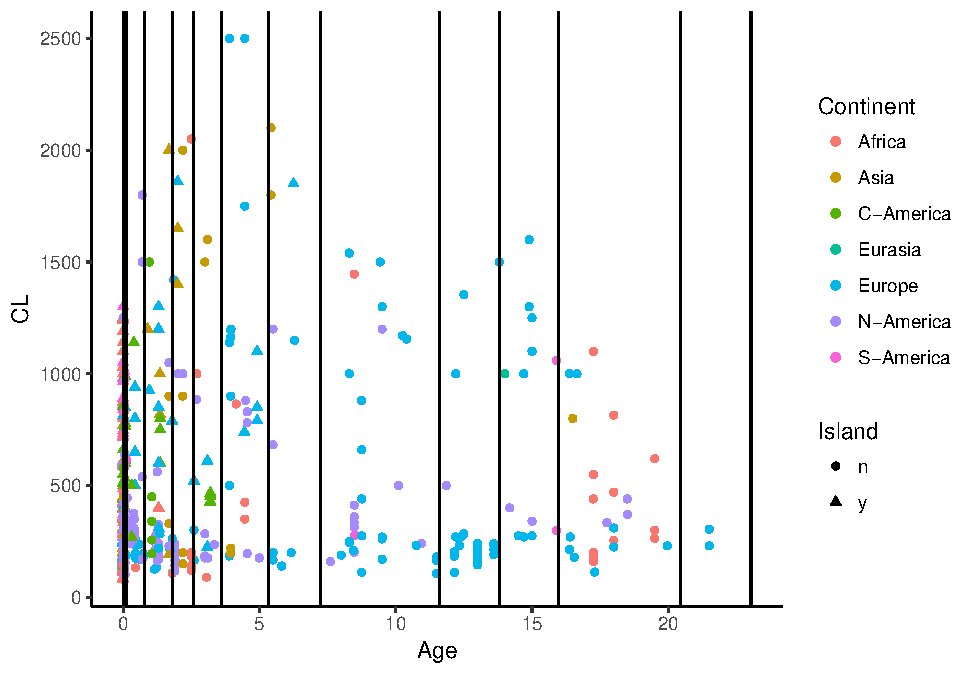
\includegraphics{MA_JJ_files/figure-latex/Get overview over data set-1.pdf}
\caption{Scatterplot of CL over time, indicating insular (triangle) and
continental (circles) and colour indicating continents. Lines indicte
bins, dashed line = new bins.}
\end{figure}

\begin{verbatim}
## [1] 0
\end{verbatim}

\newpage

\section{Maps}\label{maps}

\subsection{fossil occurences of
testudinidae}\label{fossil-occurences-of-testudinidae}

\begin{figure}[htbp]
\centering
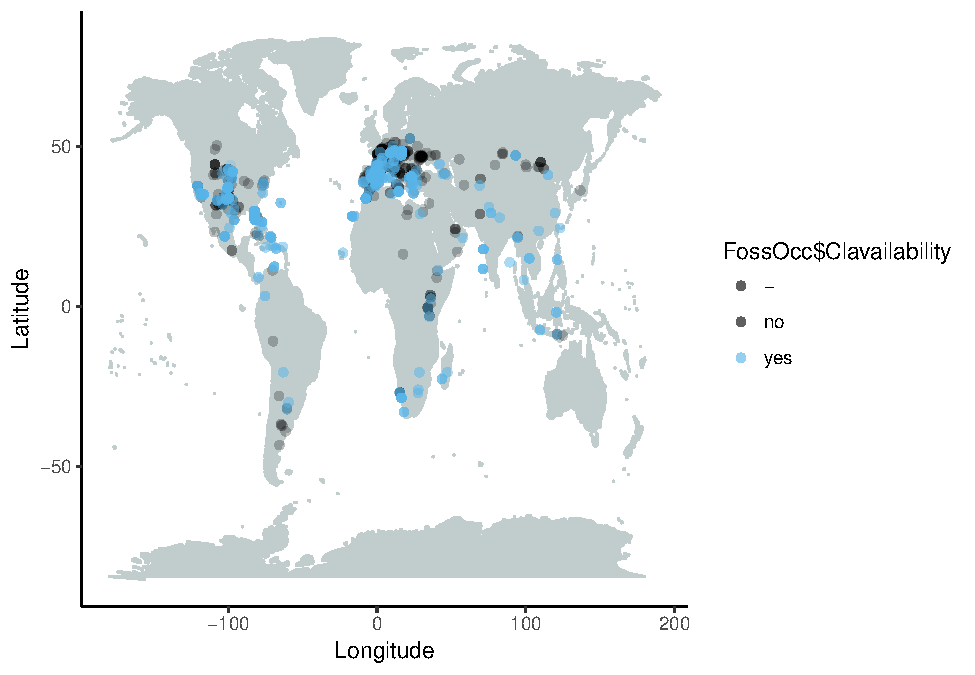
\includegraphics{MA_JJ_files/figure-latex/Map fossil occurrences-1.pdf}
\caption{Map displaying all fossil occurrences of testudinids, with
color indicating whether relevant literature was available (black if
not) and if it was, whether body size data was available or not (yes and
no, respectively).}
\end{figure}

\newpage

\subsection{body size of testudinidae}\label{body-size-of-testudinidae}

\begin{figure}[htbp]
\centering
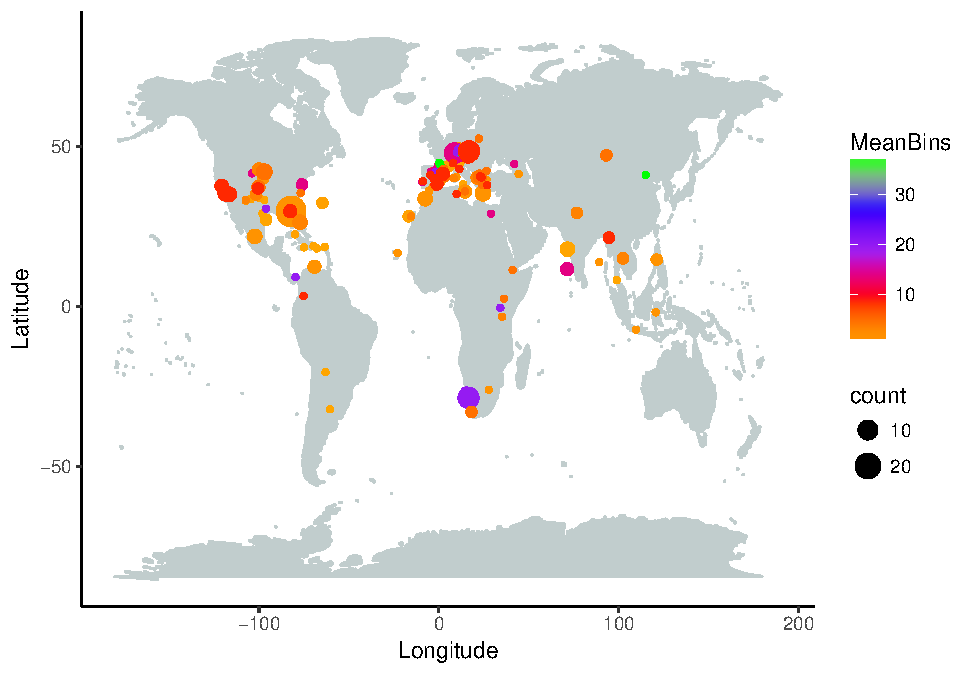
\includegraphics{MA_JJ_files/figure-latex/Map body size data set-1.pdf}
\caption{Map displaying all localities for which body size data for
testudinids was available in the literature. Size of points denotes
sample size, color denotes approximate age.}
\end{figure}

\newpage

\section{Sampling Accumulation
Curves}\label{sampling-accumulation-curves}

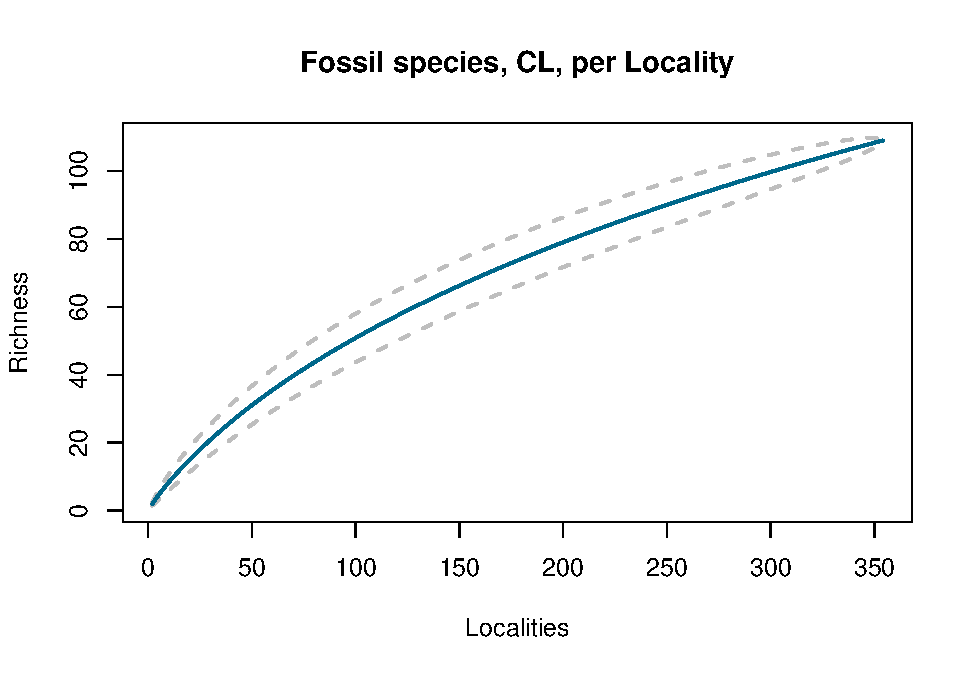
\includegraphics{MA_JJ_files/figure-latex/Species Accumulation Curve-1.pdf}
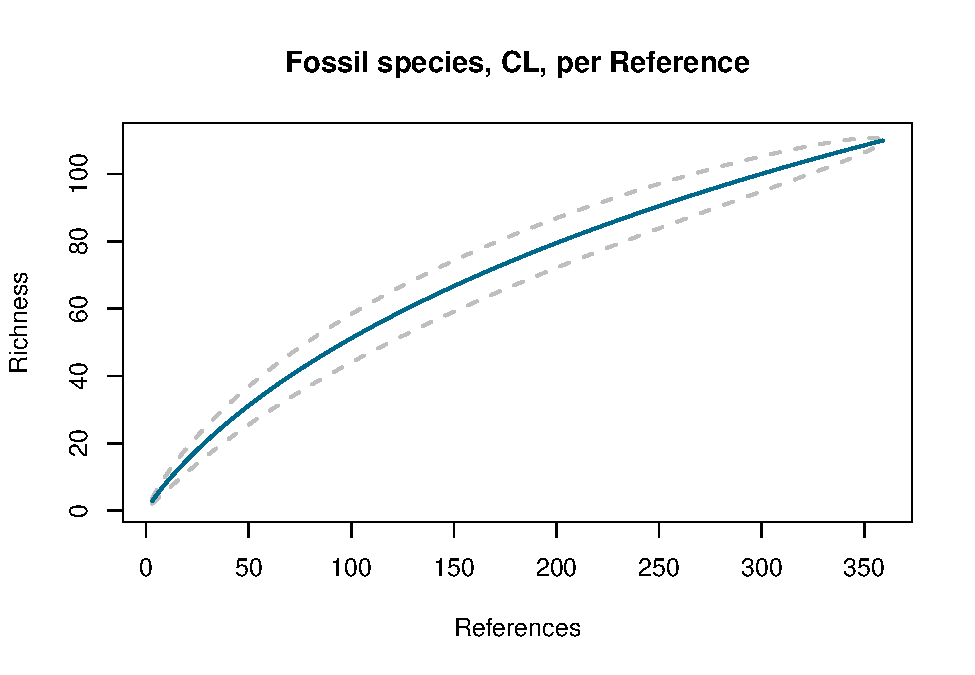
\includegraphics{MA_JJ_files/figure-latex/Species Accumulation Curve-2.pdf}

\begin{figure}[htbp]
\centering
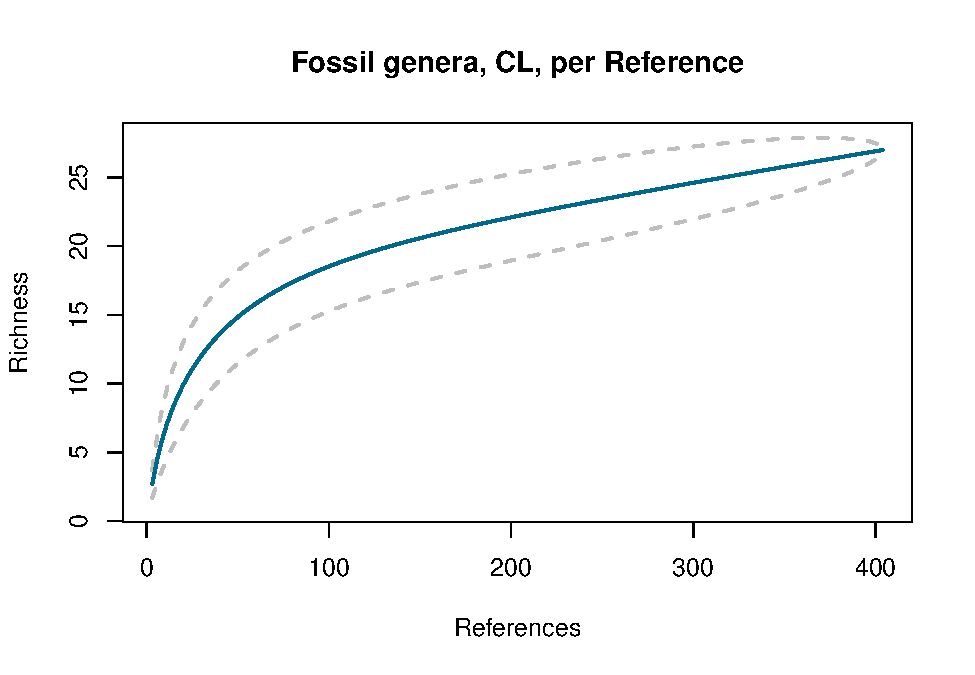
\includegraphics{MA_JJ_files/figure-latex/Species Accumulation Curve with Genera-1.pdf}
\caption{Sampling Accumulation Curve of fossil genera per reference}
\end{figure}

\begin{figure}[htbp]
\centering
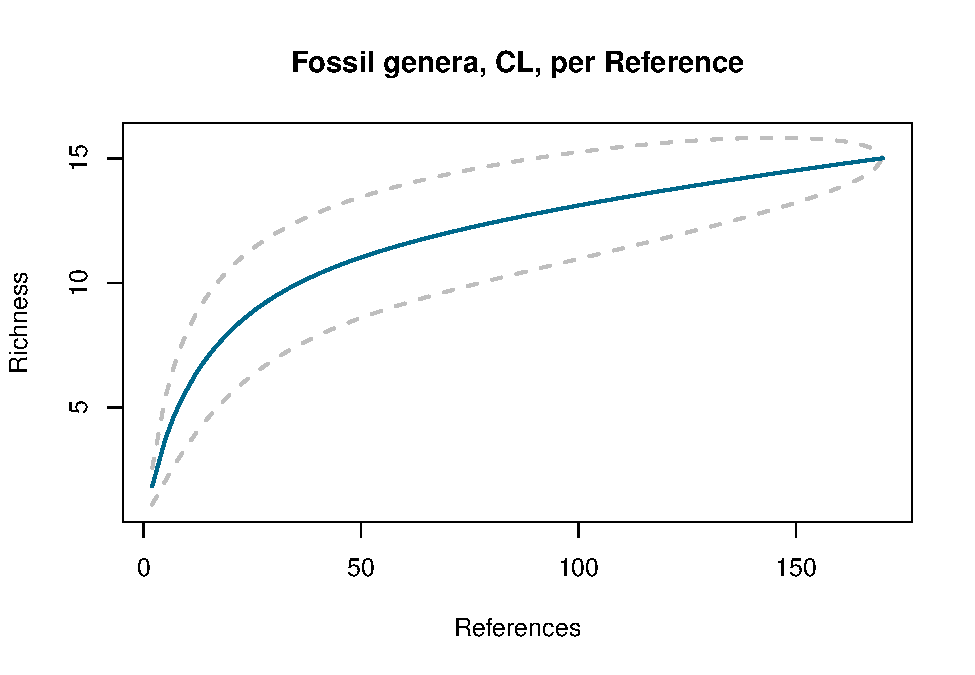
\includegraphics{MA_JJ_files/figure-latex/Species Accumulation Curve with Genera, Eurasia-1.pdf}
\caption{Sampling Accumulation Curve of fossil genera per reference,
Eurasia}
\end{figure}

\begin{figure}[htbp]
\centering
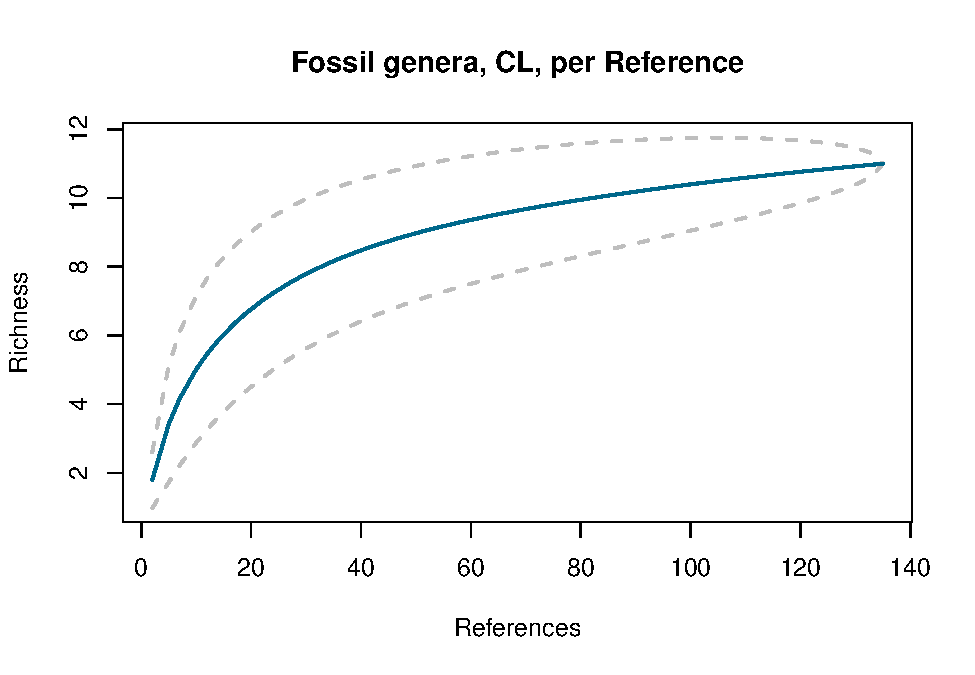
\includegraphics{MA_JJ_files/figure-latex/Species Accumulation Curve with Genera, Europe-1.pdf}
\caption{Sampling Accumulation Curve of fossil genera per reference,
Europe}
\end{figure}

\begin{figure}[htbp]
\centering
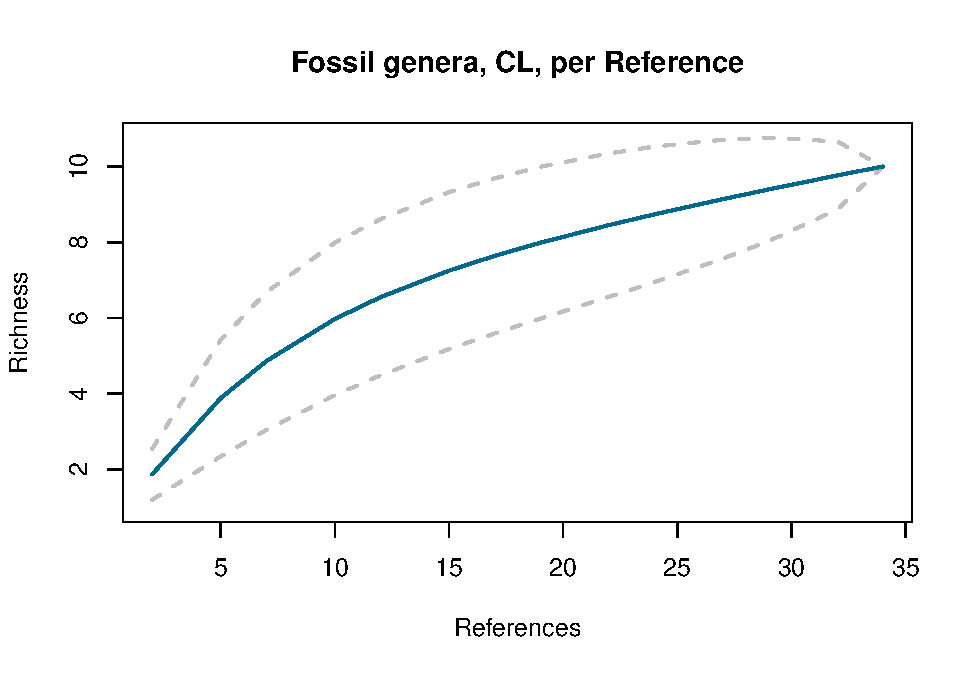
\includegraphics{MA_JJ_files/figure-latex/Species Accumulation Curve with Genera, Africa-1.pdf}
\caption{Sampling Accumulation Curve of fossil genera per reference,
Africa}
\end{figure}

\begin{figure}[htbp]
\centering
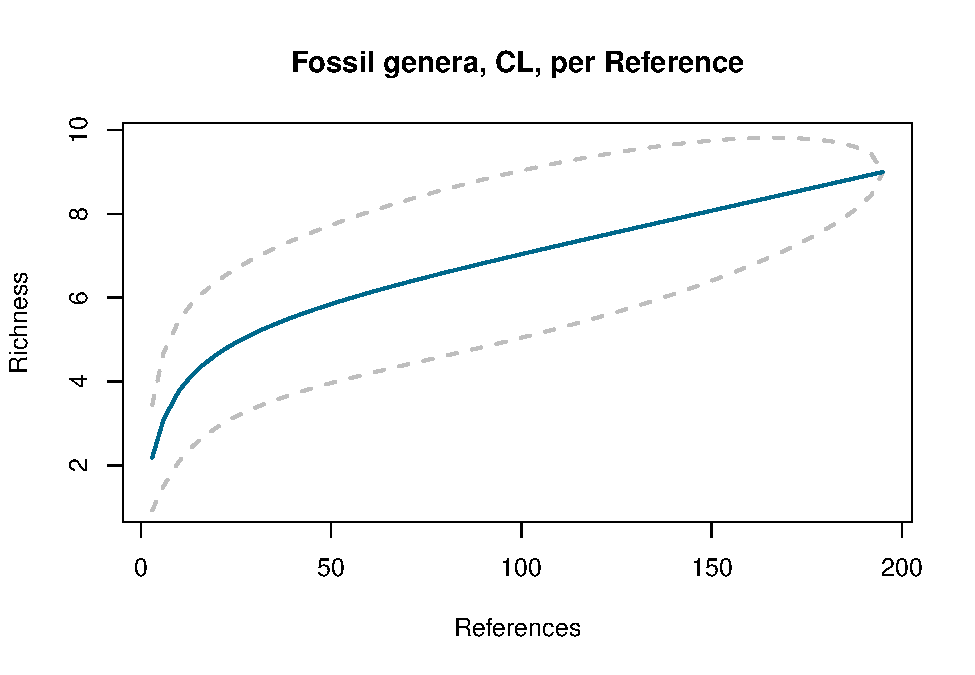
\includegraphics{MA_JJ_files/figure-latex/Species Accumulation Curve with Genera, America-1.pdf}
\caption{Sampling Accumulation Curve of fossil genera per reference,
America}
\end{figure}

\begin{figure}[htbp]
\centering
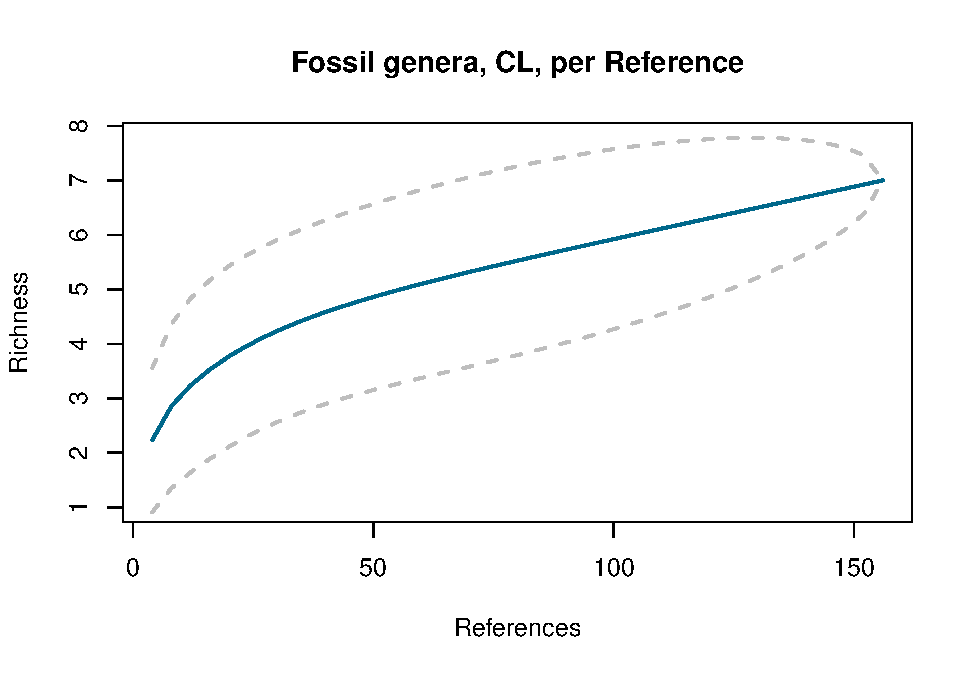
\includegraphics{MA_JJ_files/figure-latex/Species Accumulation Curve with Genera, N-America-1.pdf}
\caption{Sampling Accumulation Curve of fossil genera per reference,
N-America}
\end{figure}

\begin{figure}[htbp]
\centering
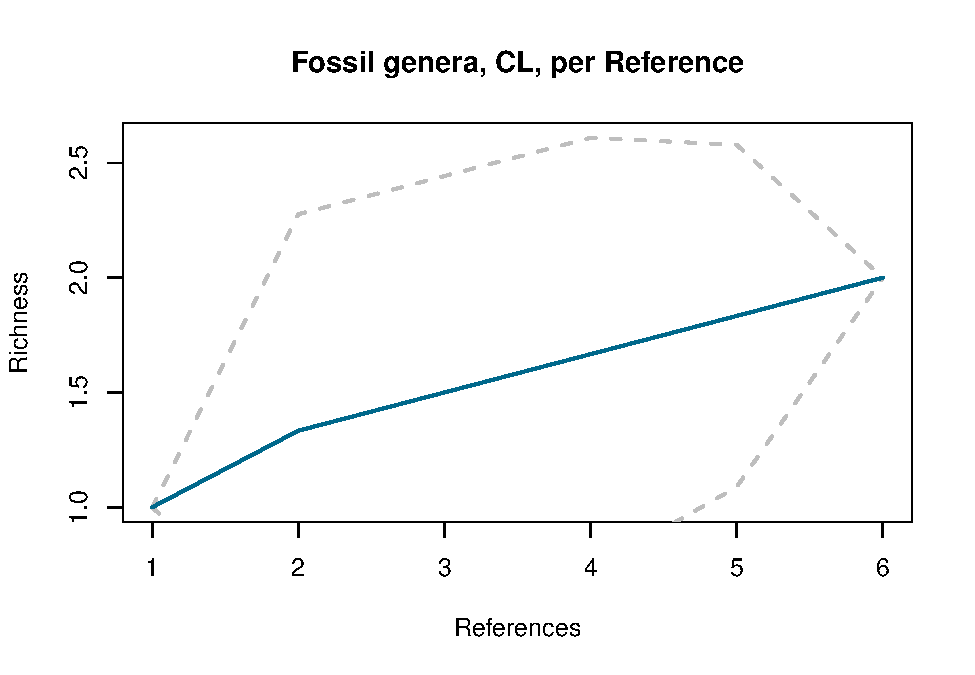
\includegraphics{MA_JJ_files/figure-latex/Species Accumulation Curve with Genera, S-America-1.pdf}
\caption{Sampling Accumulation Curve of fossil genera per reference,
S-America}
\end{figure}

\begin{figure}[htbp]
\centering
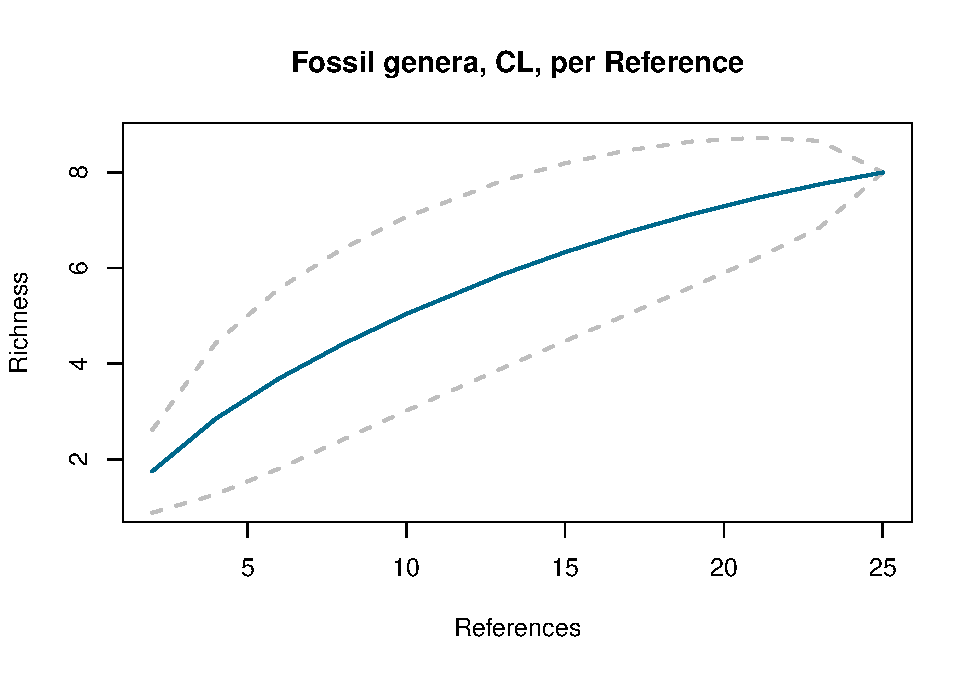
\includegraphics{MA_JJ_files/figure-latex/Species Accumulation Curve with Genera, Asia-1.pdf}
\caption{Sampling Accumulation Curve of fossil genera per reference,
Asia}
\end{figure}

\newpage

\section{Histograms}\label{histograms}

\subsection{all}\label{all}

\begin{verbatim}
## `stat_bin()` using `bins = 30`. Pick better value with `binwidth`.
\end{verbatim}

\begin{figure}[htbp]
\centering
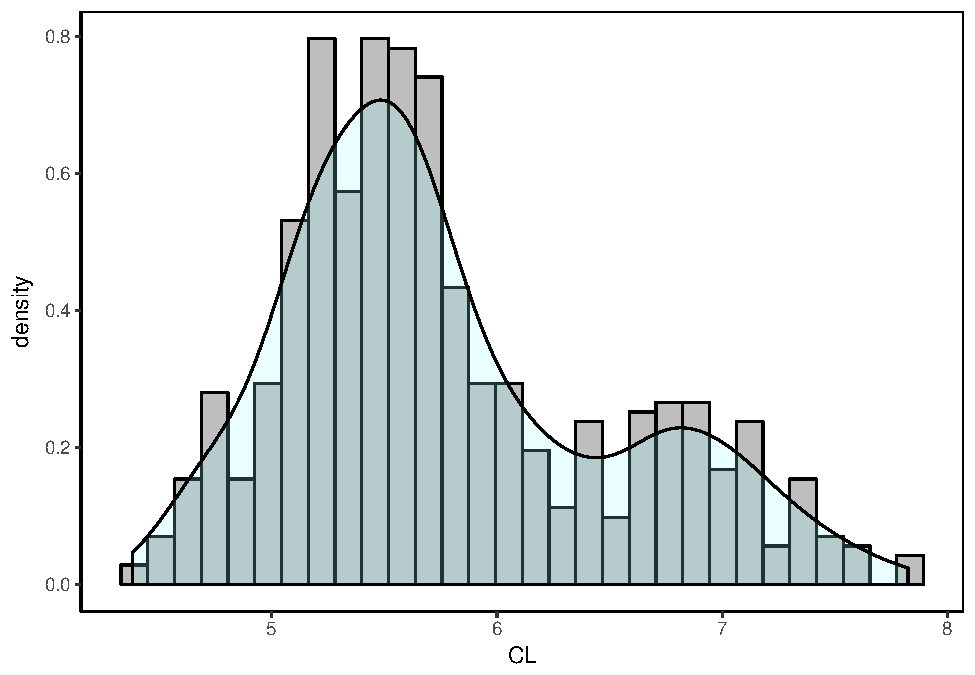
\includegraphics{MA_JJ_files/figure-latex/Histograms of body size data, all-1.pdf}
\caption{Distribution of body size data, logtransformed, all data.}
\end{figure}

\begin{Shaded}
\begin{Highlighting}[]
\KeywordTok{qqnorm}\NormalTok{(PleiPlioCL$CL); }\KeywordTok{qqline}\NormalTok{(PleiPlioCL$CL, }\DataTypeTok{col=}\DecValTok{2}\NormalTok{)}
\end{Highlighting}
\end{Shaded}

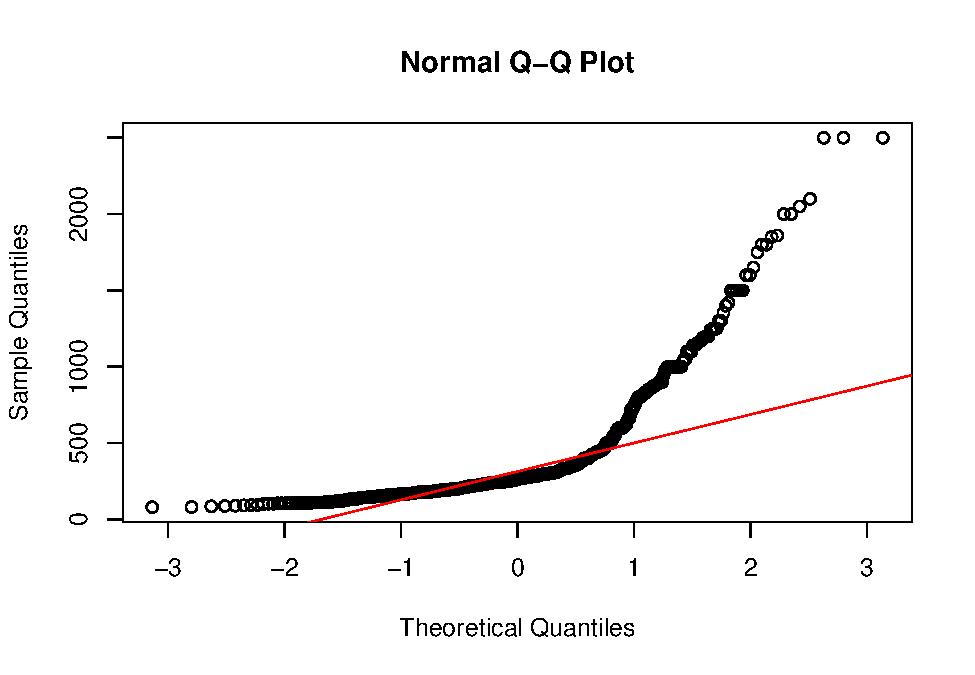
\includegraphics{MA_JJ_files/figure-latex/normal distribution, echo=FALSE-1.pdf}

\begin{Shaded}
\begin{Highlighting}[]
\KeywordTok{qqnorm}\NormalTok{(}\KeywordTok{log10}\NormalTok{(PleiPlioCL$CL)); }\KeywordTok{qqline}\NormalTok{(}\KeywordTok{log10}\NormalTok{(PleiPlioCL$CL), }\DataTypeTok{col=}\DecValTok{2}\NormalTok{)}
\end{Highlighting}
\end{Shaded}

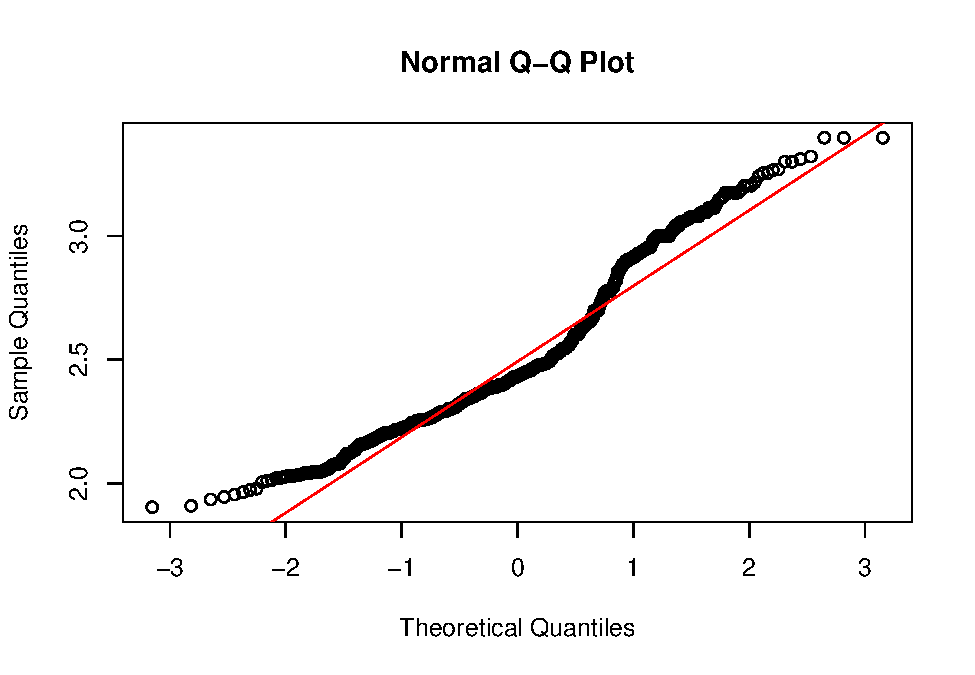
\includegraphics{MA_JJ_files/figure-latex/normal distribution, echo=FALSE-2.pdf}

\newpage

\subsection{per time bin}\label{per-time-bin}

\begin{verbatim}
## `stat_bin()` using `bins = 30`. Pick better value with `binwidth`.
\end{verbatim}

\begin{figure}[htbp]
\centering
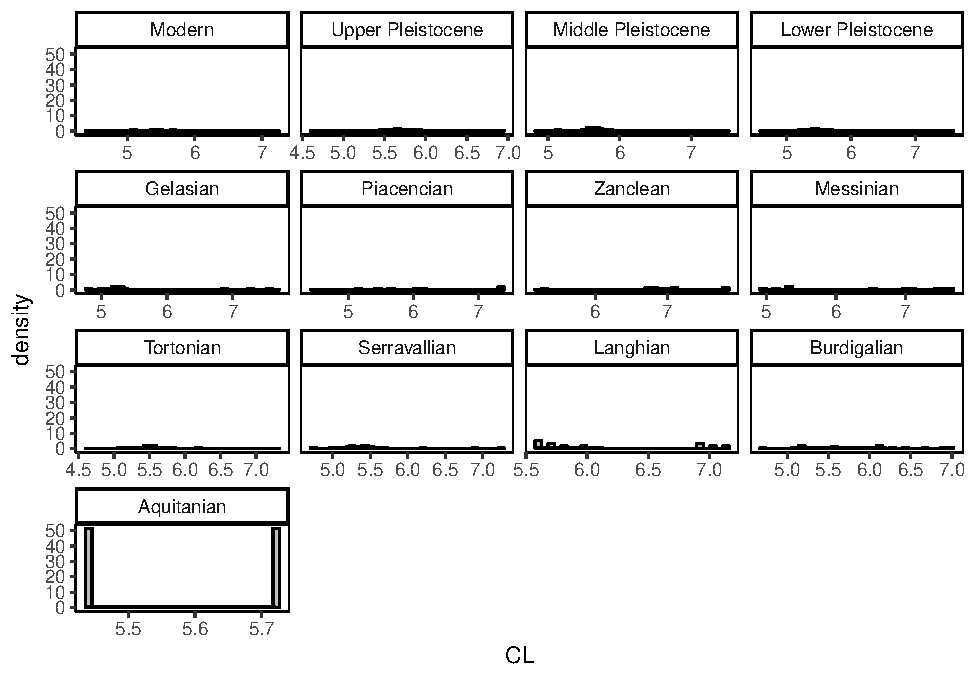
\includegraphics{MA_JJ_files/figure-latex/Histograms of body size data, per time bin-1.pdf}
\caption{Distribution of body size data per time bin, logtransformed.}
\end{figure}

\newpage

\subsection{modern vs.~fossil}\label{modern-vs.fossil}

\begin{verbatim}
## `stat_bin()` using `bins = 30`. Pick better value with `binwidth`.
\end{verbatim}

\begin{figure}[htbp]
\centering
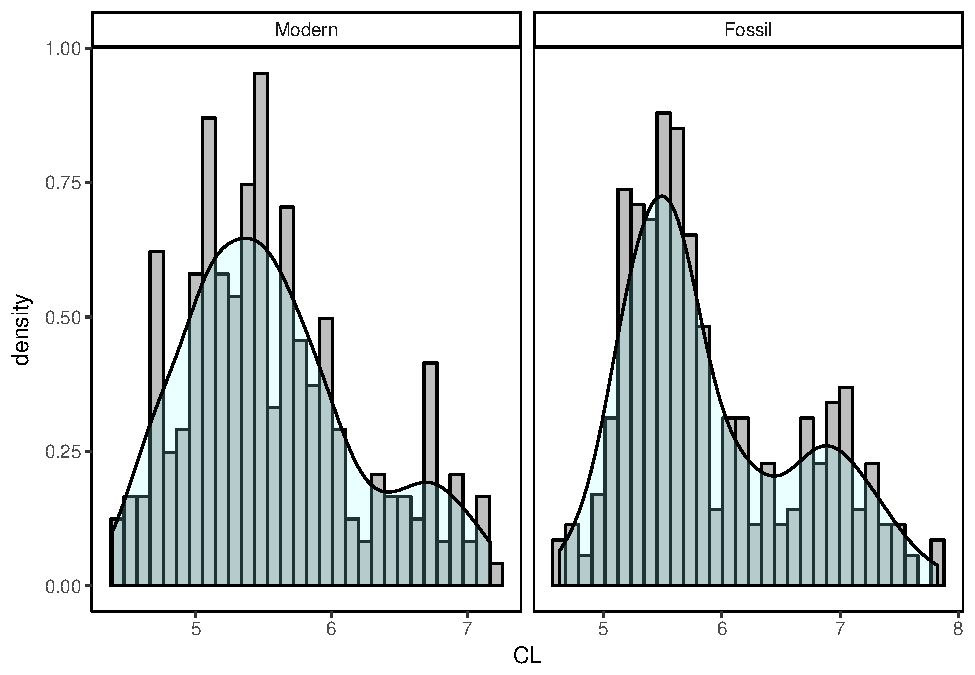
\includegraphics{MA_JJ_files/figure-latex/Histograms of body size data, modern vs. fossil-1.pdf}
\caption{Distribution of body size data modern vs.~fossil,
logtransformed.}
\end{figure}

\newpage

\subsection{modern vs.~fossil, continental
vs.~insular}\label{modern-vs.fossil-continental-vs.insular}

\begin{verbatim}
## `stat_bin()` using `bins = 30`. Pick better value with `binwidth`.
\end{verbatim}

\begin{figure}[htbp]
\centering
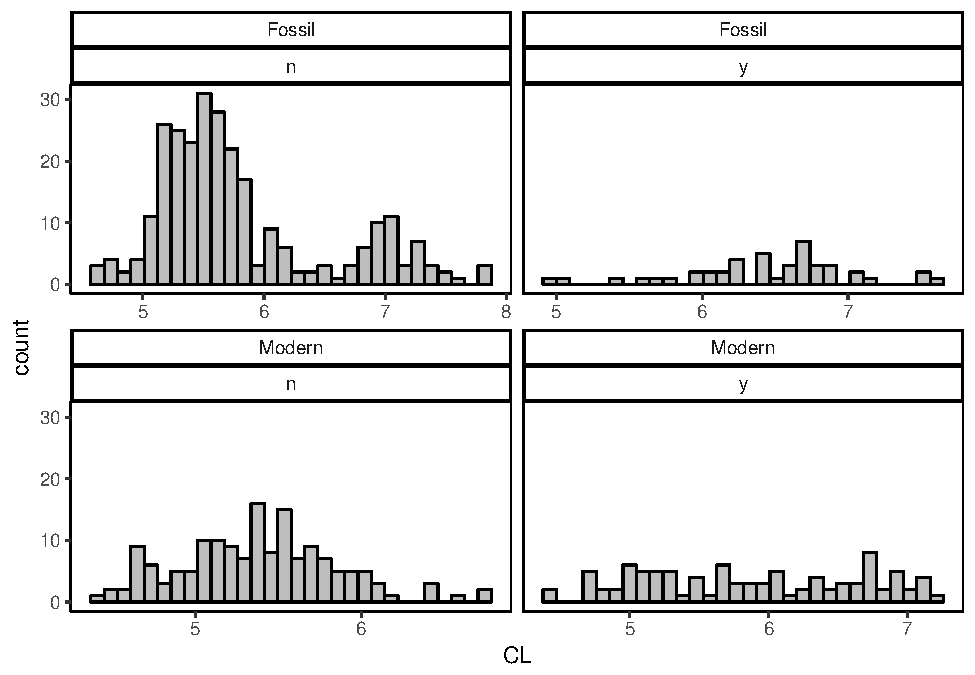
\includegraphics{MA_JJ_files/figure-latex/Histograms of body size data, modern vs. fossil, continental vs. insular-1.pdf}
\caption{Distribution of body size data modern vs.~fossil, continental
vs.~insular logtransformed.}
\end{figure}

\newpage

\subsection{continental vs.~insular}\label{continental-vs.insular}

\begin{verbatim}
## `stat_bin()` using `bins = 30`. Pick better value with `binwidth`.
\end{verbatim}

\begin{figure}[htbp]
\centering
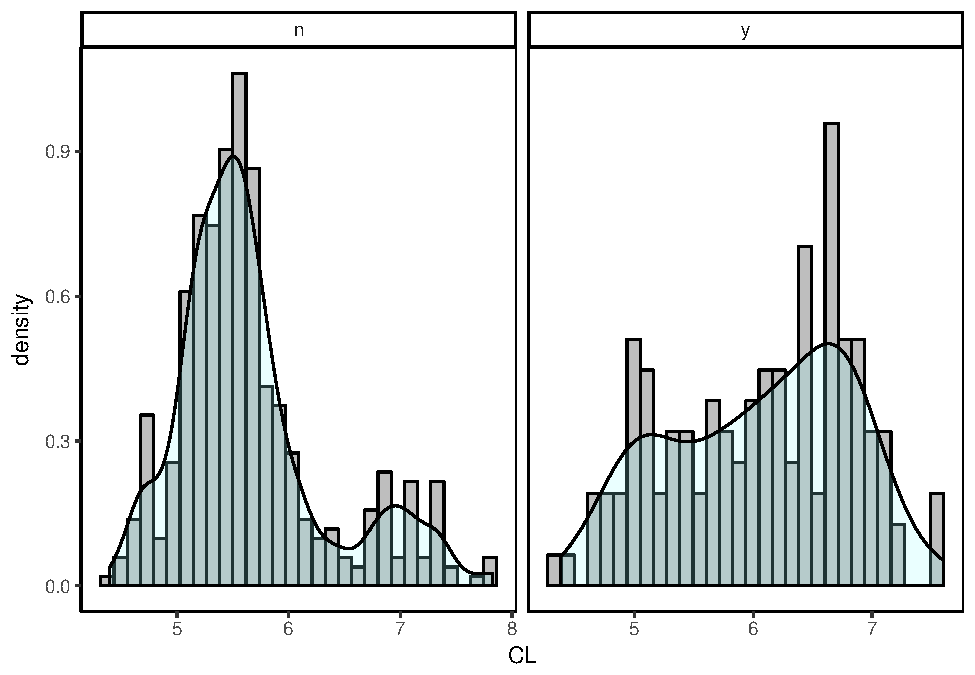
\includegraphics{MA_JJ_files/figure-latex/Histograms of body size data, continental vs. insular-1.pdf}
\caption{Distribution of body site data of continental (n) and
insular(y) species, logtransformed.}
\end{figure}

\newpage

\subsection{continents}\label{continents}

\begin{verbatim}
## `stat_bin()` using `bins = 30`. Pick better value with `binwidth`.
\end{verbatim}

\begin{figure}[htbp]
\centering
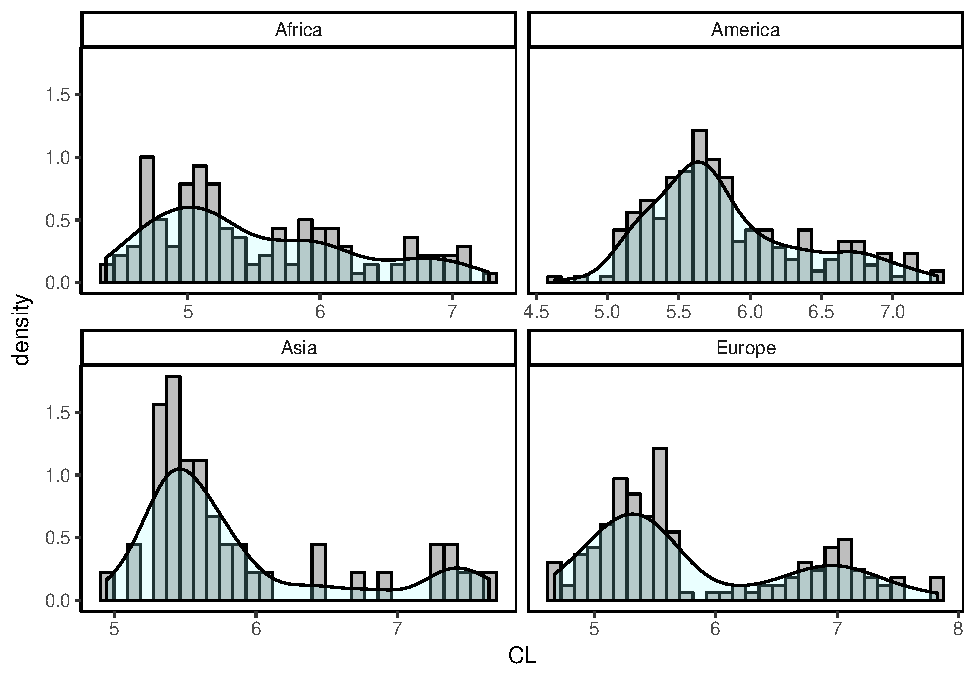
\includegraphics{MA_JJ_files/figure-latex/Histograms of body size data, split by continents-1.pdf}
\caption{Distribution of body site data per continent, logtransformed.}
\end{figure}

\newpage

\subsection{General statistics}\label{general-statistics}

\begin{longtable}[]{@{}rrrrrrrrrrrrl@{}}
\caption{General statistics of body size data: all, per time bin,
insular and continental, per continent (all referring to CL: min, max,
variance, mean, logmean, median, logmedian, skewness, logskewness,
kurosis, logkurtosis}\tabularnewline
\toprule
nCL & min & max & var & mean & logm & med & logmed & skew & logsk & kurt
& logku & Variable\tabularnewline
\midrule
\endfirsthead
\toprule
nCL & min & max & var & mean & logm & med & logmed & skew & logsk & kurt
& logku & Variable\tabularnewline
\midrule
\endhead
616 & 80.00 & 2500 & 164537.80 & 437.2 & 2.5 & 270.5 & 2.4 & 2.14 & 0.69
& 8.00 & 2.73 & all\tabularnewline
253 & 80.00 & 1300 & 67485.50 & 330.3 & 2.4 & 242.0 & 2.4 & 1.83 & 0.58
& 5.87 & 2.69 & Modern\tabularnewline
49 & 102.44 & 1250 & 69690.66 & 445.9 & 2.6 & 334.7 & 2.5 & 1.20 & 0.24
& 3.61 & 2.56 & Upper Pleistocene\tabularnewline
53 & 132.00 & 1800 & 97910.83 & 387.1 & 2.5 & 292.9 & 2.5 & 3.03 & 1.52
& 12.24 & 5.55 & Middle Pleistocene\tabularnewline
57 & 107.80 & 2000 & 161948.82 & 463.5 & 2.5 & 263.0 & 2.4 & 1.74 & 0.73
& 5.76 & 2.40 & Lower Pleistocene\tabularnewline
31 & 118.90 & 2050 & 411224.51 & 555.2 & 2.5 & 194.9 & 2.3 & 1.31 & 0.93
& 3.12 & 2.11 & Gelasian\tabularnewline
21 & 90.00 & 1600 & 270535.82 & 610.6 & 2.6 & 428.0 & 2.6 & 1.00 & 0.14
& 2.50 & 1.99 & Piacencian\tabularnewline
26 & 176.00 & 2500 & 476162.71 & 955.2 & 2.9 & 857.5 & 2.9 & 1.11 &
-0.40 & 3.56 & 2.30 & Zanclean\tabularnewline
10 & 140.00 & 2100 & 602611.21 & 948.9 & 2.8 & 916.0 & 2.9 & 0.26 &
-0.22 & 1.49 & 1.29 & Messinian\tabularnewline
45 & 107.00 & 1540 & 175470.12 & 462.7 & 2.5 & 250.0 & 2.4 & 1.49 & 0.81
& 3.74 & 2.54 & Tortonian\tabularnewline
27 & 111.00 & 1500 & 126060.40 & 337.7 & 2.4 & 220.0 & 2.3 & 2.49 & 1.77
& 7.77 & 5.30 & Serravallian\tabularnewline
14 & 270.00 & 1600 & 230451.33 & 747.9 & 2.8 & 700.0 & 2.8 & 0.30 & 0.03
& 1.55 & 1.18 & Langhian\tabularnewline
30 & 113.00 & 1100 & 76288.76 & 406.8 & 2.5 & 302.4 & 2.5 & 1.27 & 0.45
& 3.45 & 2.26 & Burdigalian/Aquitanian\tabularnewline
253 & 80.00 & 1300 & 67485.50 & 330.3 & 2.4 & 242.0 & 2.4 & 1.83 & 0.58
& 5.87 & 2.69 & Modern\tabularnewline
363 & 90.00 & 2500 & 219004.66 & 511.7 & 2.6 & 285.6 & 2.5 & 1.83 & 0.68
& 6.11 & 2.42 & Fossil\tabularnewline
469 & 81.00 & 2500 & 157808.79 & 392.9 & 2.5 & 250.0 & 2.4 & 2.65 & 1.07
& 10.57 & 3.74 & continental\tabularnewline
147 & 80.00 & 2000 & 160834.35 & 578.5 & 2.6 & 500.0 & 2.7 & 1.02 &
-0.27 & 3.95 & 2.05 & insular\tabularnewline
157 & 81.00 & 830 & 17009.02 & 244.0 & 2.3 & 221.0 & 2.3 & 1.92 & 0.29 &
8.09 & 2.98 & modern-con\tabularnewline
96 & 80.00 & 1300 & 118641.09 & 471.5 & 2.6 & 353.0 & 2.5 & 0.82 & 0.01
& 2.47 & 1.77 & modern-ins\tabularnewline
312 & 90.00 & 2500 & 212116.79 & 467.9 & 2.5 & 270.0 & 2.4 & 2.11 & 0.96
& 7.25 & 2.96 & fossil-con\tabularnewline
51 & 150.00 & 2000 & 180825.40 & 780.0 & 2.8 & 750.0 & 2.9 & 1.11 &
-0.40 & 4.02 & 3.18 & fossil-ins\tabularnewline
142 & 80.00 & 2050 & 112417.26 & 347.7 & 2.4 & 193.5 & 2.3 & 2.10 & 0.68
& 7.97 & 2.48 & Africa\tabularnewline
242 & 102.44 & 1800 & 82209.71 & 415.0 & 2.5 & 302.2 & 2.5 & 1.92 & 0.75
& 6.79 & 2.91 & America\tabularnewline
59 & 150.00 & 2100 & 323123.20 & 585.5 & 2.6 & 280.0 & 2.4 & 1.43 & 0.85
& 3.61 & 2.24 & Asia\tabularnewline
173 & 107.00 & 2500 & 254222.84 & 491.2 & 2.5 & 245.0 & 2.4 & 1.86 &
0.81 & 6.30 & 2.34 & Europe\tabularnewline
\bottomrule
\end{longtable}

\newpage

\section{Boxplots}\label{boxplots}

\subsection{genera per time bins}\label{genera-per-time-bins}

\begin{figure}[htbp]
\centering
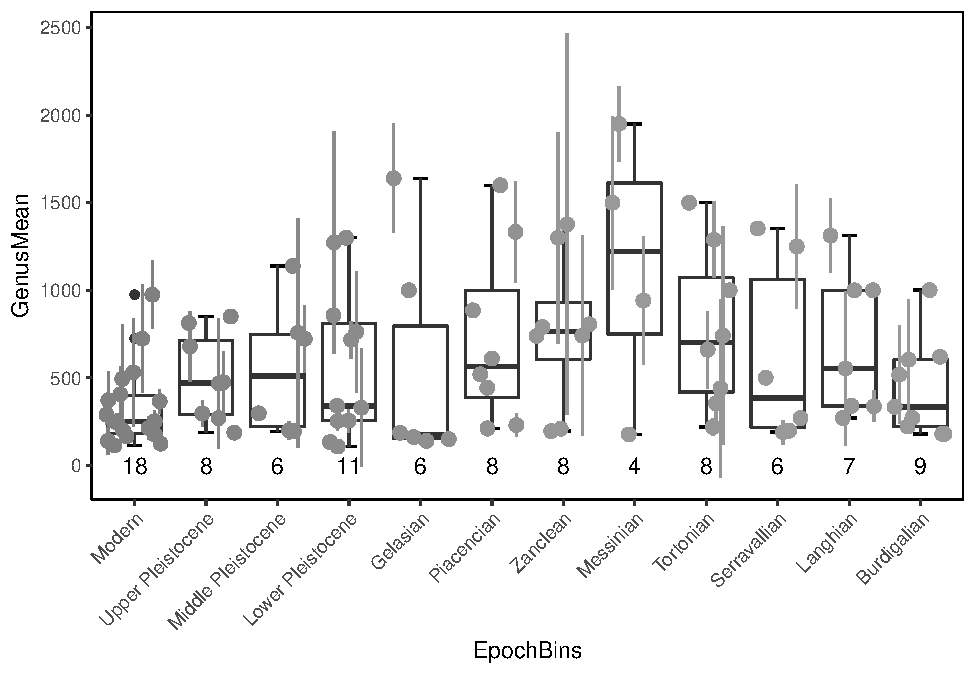
\includegraphics{MA_JJ_files/figure-latex/Boxplots of each genus per time bin-1.pdf}
\caption{Boxplots of mean CL per time bin, including mean and sd CL for
each genus (as pointrange).}
\end{figure}

\newpage

\subsection{continental vs.~insular per time
bin}\label{continental-vs.insular-per-time-bin}

\begin{figure}[htbp]
\centering
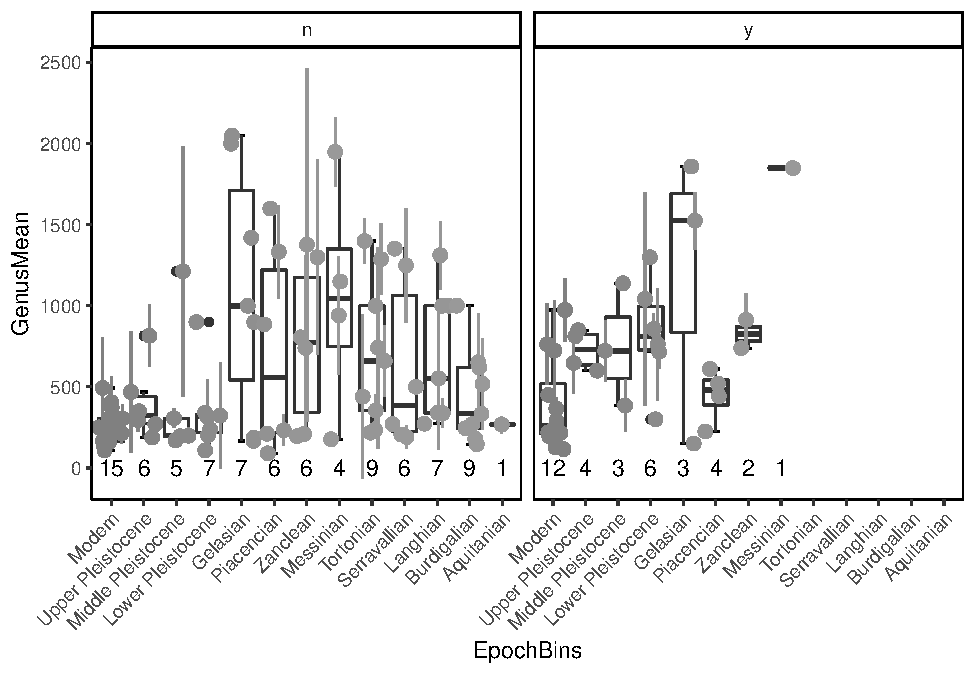
\includegraphics{MA_JJ_files/figure-latex/Boxplots of each genus per time bin, continental vs. insular-1.pdf}
\caption{Boxplots of each genus per time bin, continental vs.~insular
species.}
\end{figure}

\newpage

\subsection{fossil vs.~modern}\label{fossil-vs.modern}

\begin{figure}[htbp]
\centering
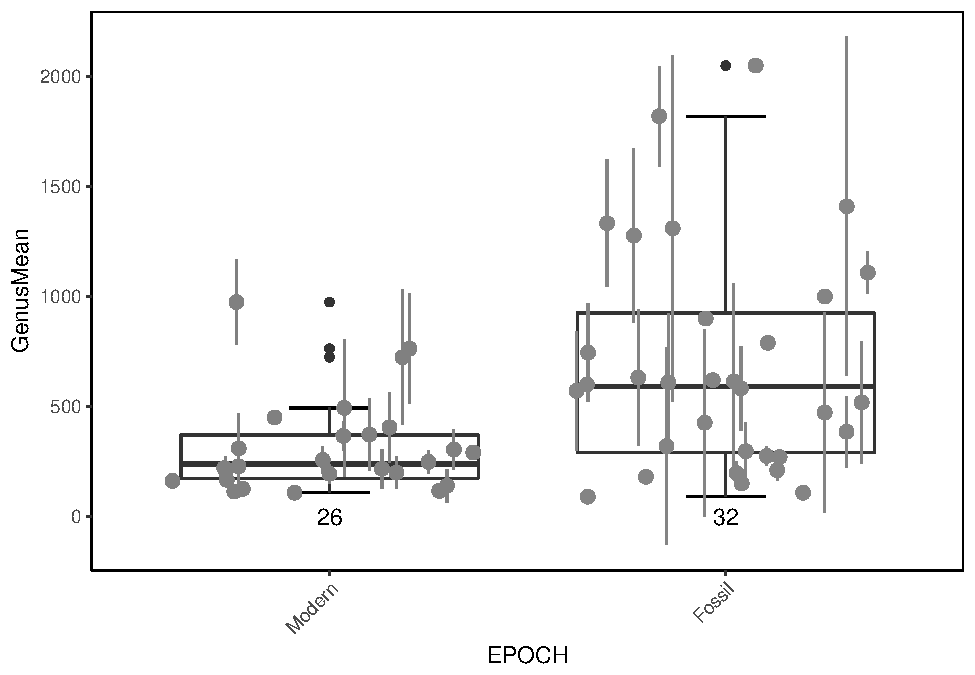
\includegraphics{MA_JJ_files/figure-latex/Boxplots modern vs. fossil-1.pdf}
\caption{Boxplots fossil vs.~modern.}
\end{figure}

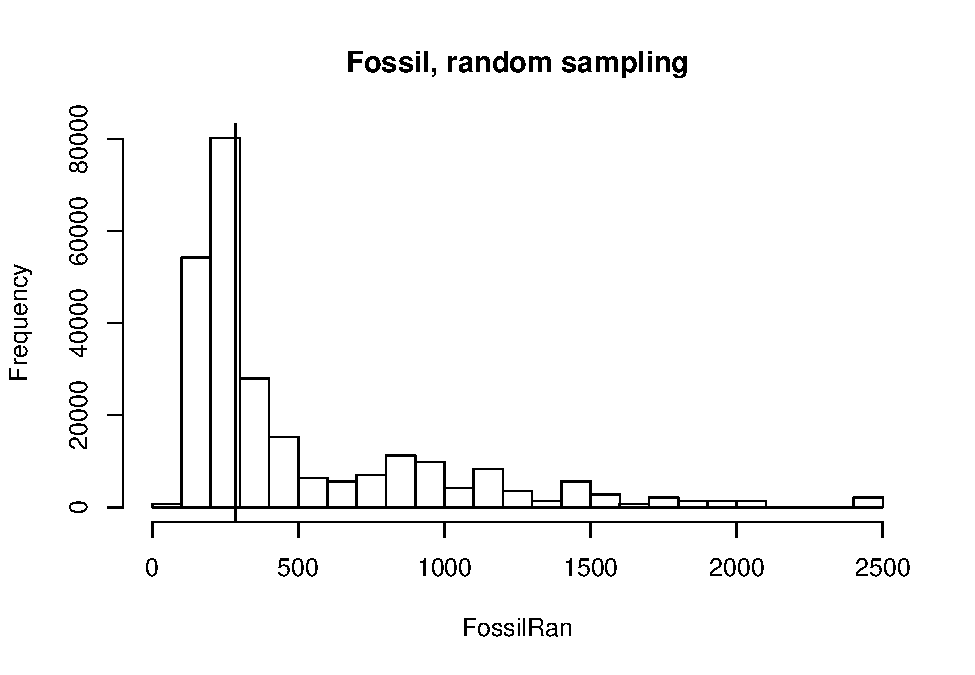
\includegraphics{MA_JJ_files/figure-latex/randon sampling modern fossil-1.pdf}

\begin{verbatim}
## [1] 330.3495
\end{verbatim}

\begin{verbatim}
## [1] 515.4103
\end{verbatim}

\begin{verbatim}
## 
##  Wilcoxon rank sum test with continuity correction
## 
## data:  Modern and Fossil
## W = 23396, p-value = 1.603e-07
## alternative hypothesis: true location shift is less than 0
\end{verbatim}

Wilcoxon Rank Sum Test (unpaired data):

modern \textless{} fossil (P = \(1.6026752\times 10^{-7}\))

\newpage

\subsection{fossil vs.~modern, continental
vs.~insular}\label{fossil-vs.modern-continental-vs.insular}

\begin{figure}[htbp]
\centering
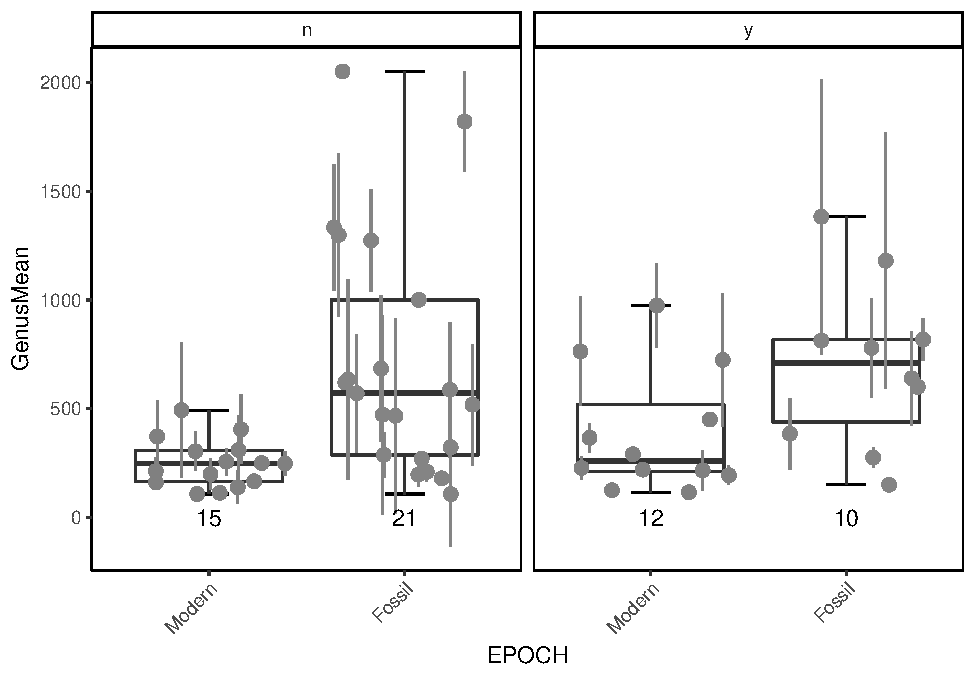
\includegraphics{MA_JJ_files/figure-latex/Boxplots fossil vs. modern, continental vs. insular-1.pdf}
\caption{Boxplots fossil vs.~modern, continental vs.~insular species.}
\end{figure}

\begin{verbatim}
## [1] 51
\end{verbatim}

\begin{verbatim}
## [1] 51
\end{verbatim}

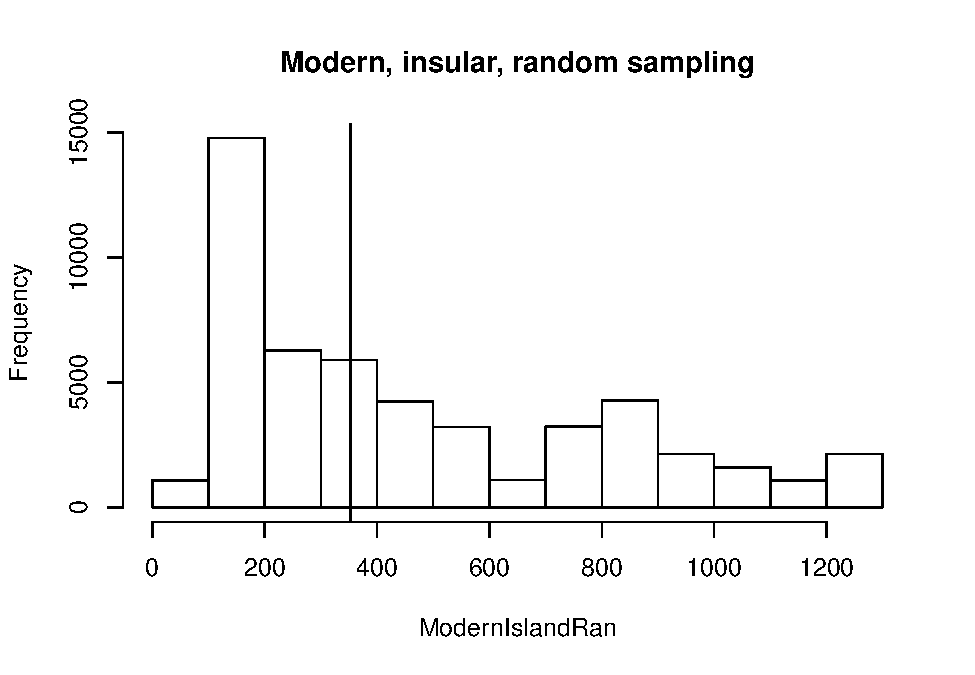
\includegraphics{MA_JJ_files/figure-latex/randon sampling modern fossil, island continental-1.pdf}

\begin{verbatim}
## 
##  Wilcoxon rank sum test with continuity correction
## 
## data:  ModernIsland and FossilIsland
## W = 758.5, p-value = 0.0001448
## alternative hypothesis: true location shift is less than 0
\end{verbatim}

\begin{verbatim}
## [1] 157
\end{verbatim}

\begin{verbatim}
## [1] 157
\end{verbatim}

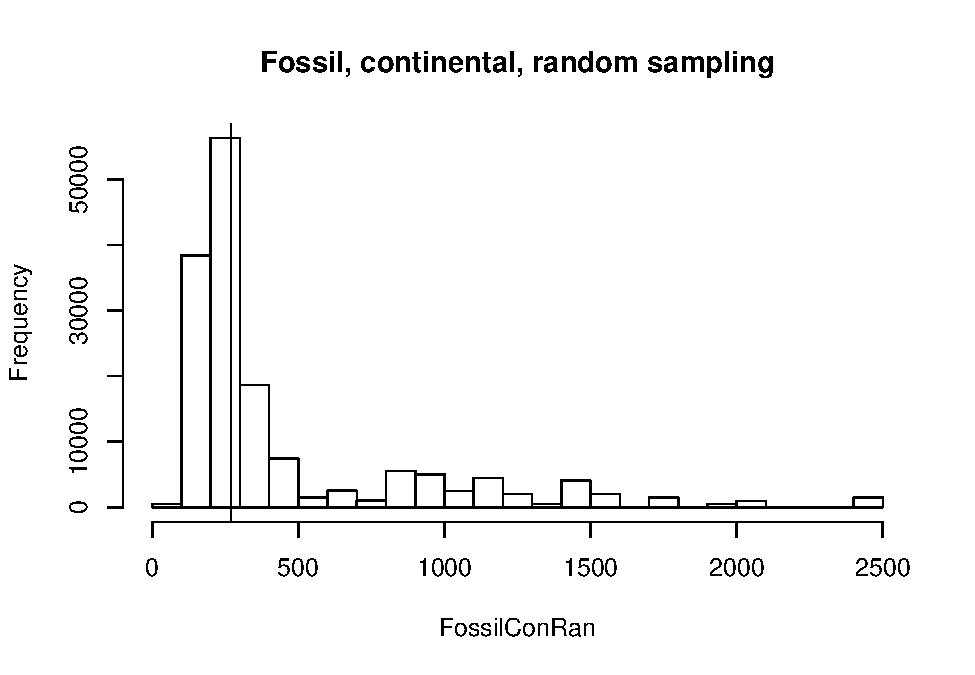
\includegraphics{MA_JJ_files/figure-latex/randon sampling modern fossil, island continental-2.pdf}

\begin{verbatim}
## 
##  Wilcoxon rank sum test with continuity correction
## 
## data:  ModernCon and FossilCon
## W = 7737.5, p-value = 5.92e-09
## alternative hypothesis: true location shift is less than 0
\end{verbatim}

Wilcoxon Rank Sum Test (unpaired data):

modern continental \textless{} fossil continental (P =
\(5.9202322\times 10^{-9}\))

modern insular \textless{} fossil insular (P =
\(1.4478883\times 10^{-4}\))

\newpage

\subsection{continental vs.~insular}\label{continental-vs.insular-1}

\begin{figure}[htbp]
\centering
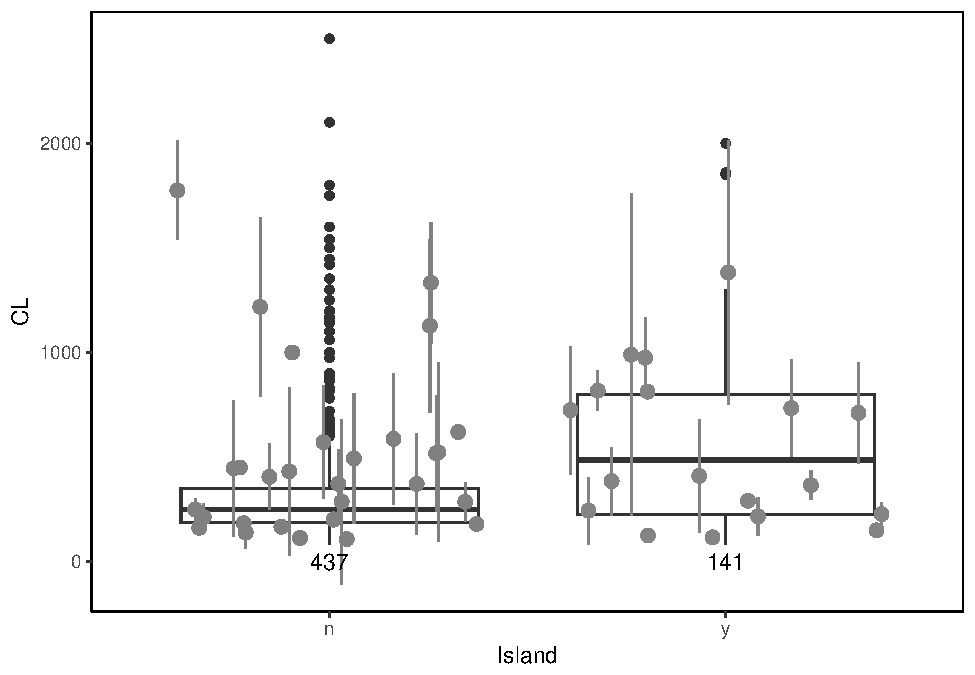
\includegraphics{MA_JJ_files/figure-latex/Boxplot continental vs. insular-1.pdf}
\caption{Boxplot continental vs.~insular, genera summarised}
\end{figure}

\begin{verbatim}
## [1] 147
\end{verbatim}

\begin{verbatim}
## [1] 147
\end{verbatim}

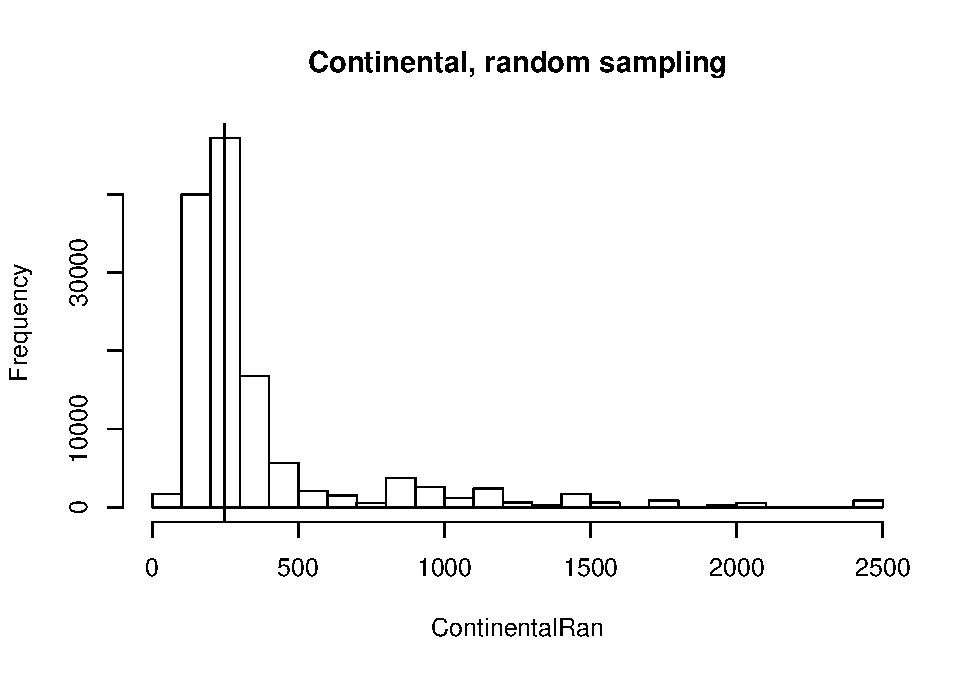
\includegraphics{MA_JJ_files/figure-latex/randon sampling island continental-1.pdf}

\begin{verbatim}
## 
##  Wilcoxon rank sum test with continuity correction
## 
## data:  Insular and Continental
## W = 14353, p-value = 5.634e-07
## alternative hypothesis: true location shift is greater than 0
\end{verbatim}

Wilcoxon Rank Sum Test (unpaired data):

continental \textless{} insular (P = \(5.6343766\times 10^{-7}\))

\newpage

\subsection{continental vs.~insular per time
bin}\label{continental-vs.insular-per-time-bin-1}

\begin{figure}[htbp]
\centering
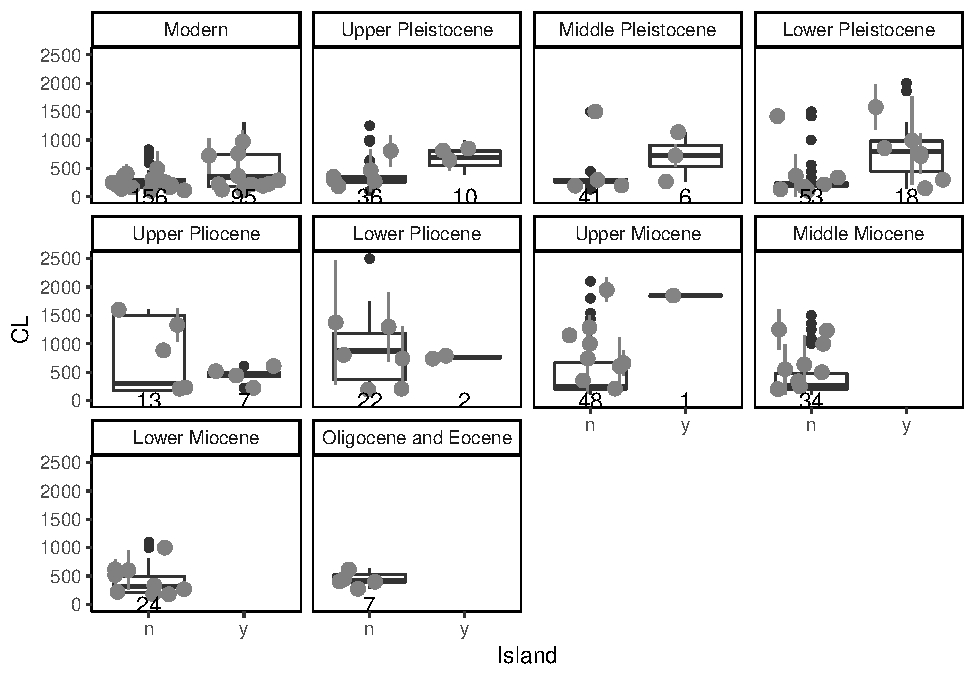
\includegraphics{MA_JJ_files/figure-latex/Boxplot continental vs. insular, split into time bins-1.pdf}
\caption{Boxplot continental vs.~insular, genera summarised}
\end{figure}

\newpage

\subsection{continents}\label{continents-1}

\begin{figure}[htbp]
\centering
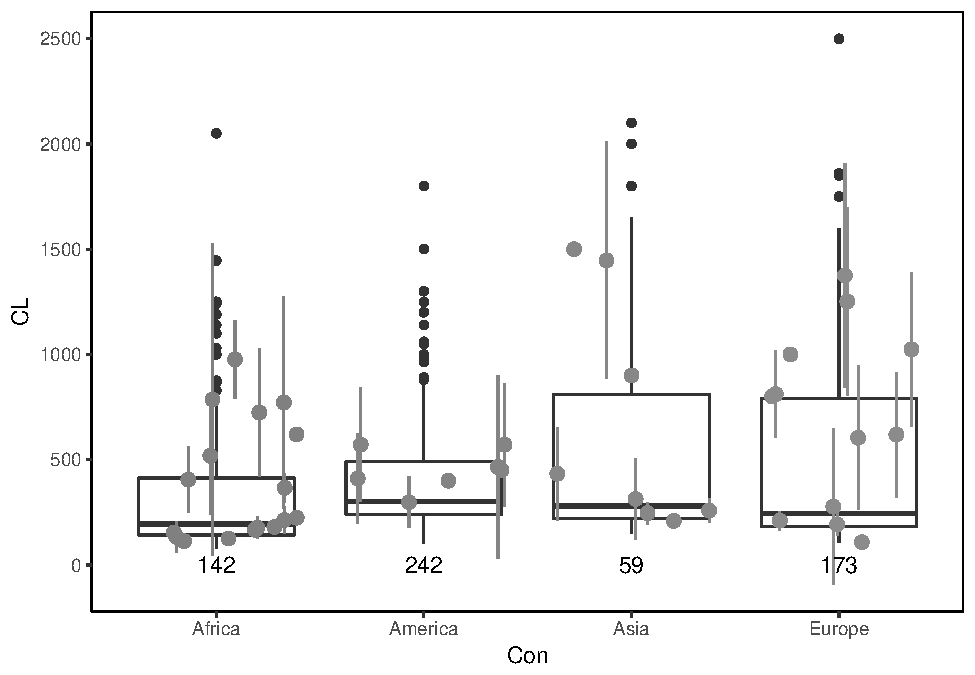
\includegraphics{MA_JJ_files/figure-latex/Boxplot body size split into continents-1.pdf}
\caption{Boxplot: body size on different continents, genera summarised}
\end{figure}

\begin{verbatim}
## [1] 142
\end{verbatim}

\begin{verbatim}
## [1] 347.6887
\end{verbatim}

\begin{verbatim}
## [1] 142
\end{verbatim}

\begin{verbatim}
## [1] 437.2697
\end{verbatim}

\begin{verbatim}
## [1] 59
\end{verbatim}

\begin{verbatim}
## [1] 173
\end{verbatim}

\begin{verbatim}
## [1] 142
\end{verbatim}

\begin{verbatim}
## [1] 515.7585
\end{verbatim}

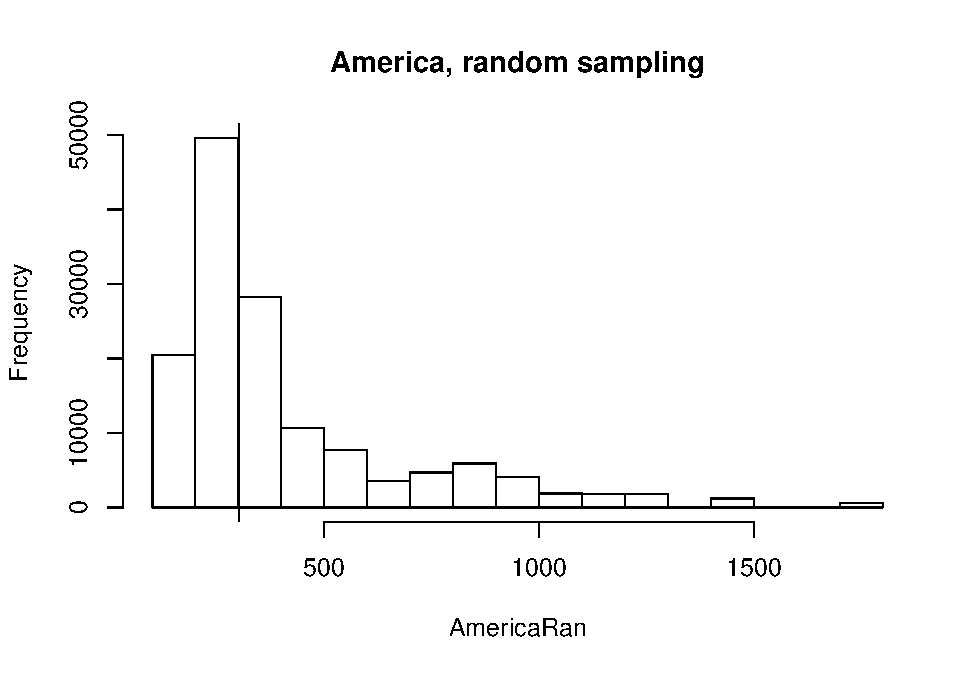
\includegraphics{MA_JJ_files/figure-latex/randon sampling continents-1.pdf}
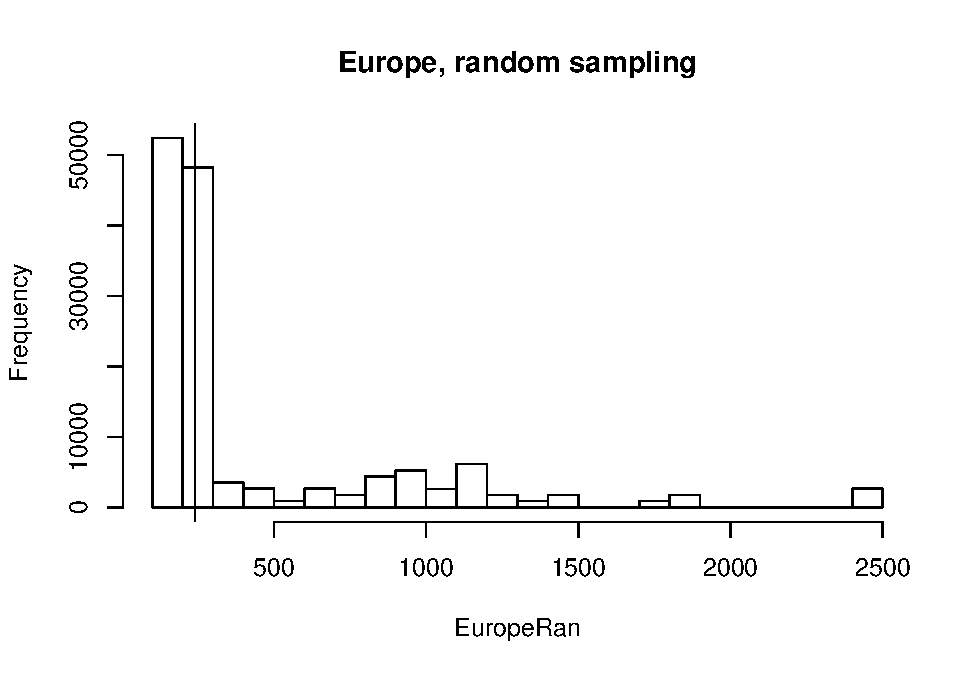
\includegraphics{MA_JJ_files/figure-latex/randon sampling continents-2.pdf}
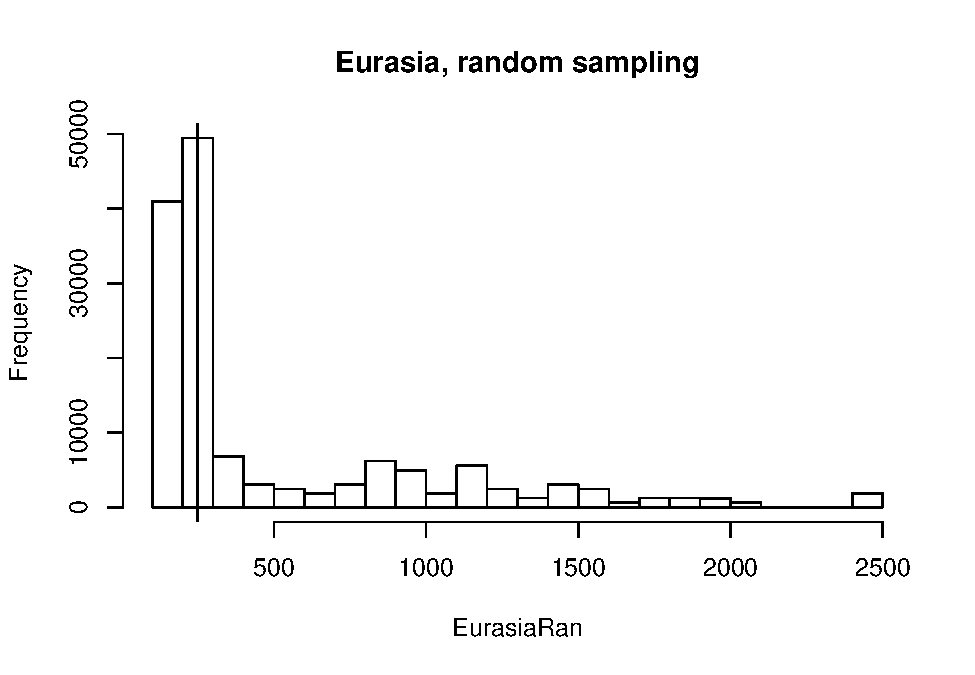
\includegraphics{MA_JJ_files/figure-latex/randon sampling continents-3.pdf}

\begin{verbatim}
## 
##  Kruskal-Wallis rank sum test
## 
## data:  list(Africa, America, Eurasia, Europe)
## Kruskal-Wallis chi-squared = 31.847, df = 3, p-value = 5.636e-07
\end{verbatim}

Kruskal-Wallis-Test:

Continent means differ (P = \(5.6359048\times 10^{-7}\)) (still have to
look into the details\ldots{})

\newpage

\subsection{continents, continental
vs.~insular}\label{continents-continental-vs.insular}

\begin{figure}[htbp]
\centering
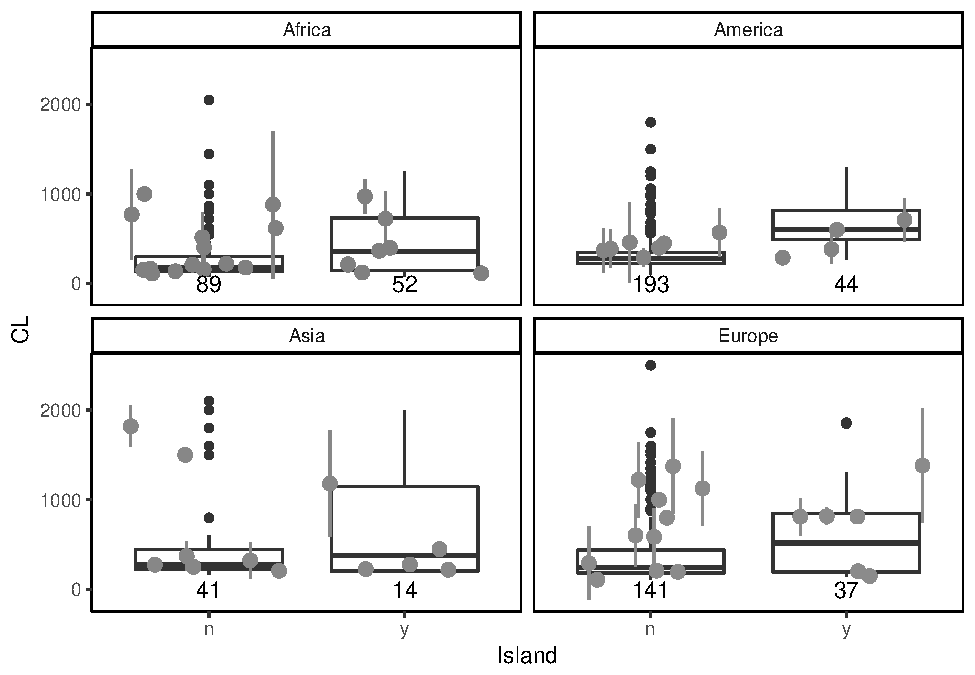
\includegraphics{MA_JJ_files/figure-latex/Boxplot body size split into continents, continental vs. insular-1.pdf}
\caption{Boxplot: body size on different continents, genera summarised}
\end{figure}

\newpage

\section{paleoTS analysis}\label{paleots-analysis}

\subsection{all (continental and
insular)}\label{all-continental-and-insular}

\subsubsection{genera (all)}\label{genera-all}

\begin{figure}[htbp]
\centering
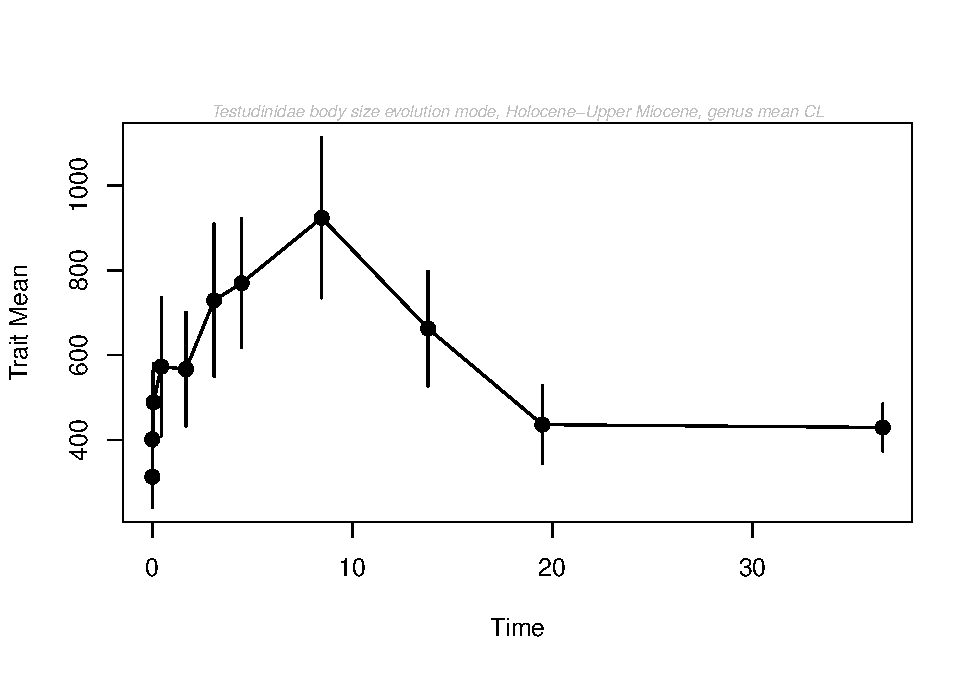
\includegraphics{MA_JJ_files/figure-latex/paleoTS plot with genus mean, including island species-1.pdf}
\caption{paleoTS plot with genus mean, including island species}
\end{figure}

\begin{longtable}[]{@{}lrrrr@{}}
\caption{Model-fitting results for testudinidae, genera, including
island species}\tabularnewline
\toprule
& logL & K & AICc & Akaike.wt\tabularnewline
\midrule
\endfirsthead
\toprule
& logL & K & AICc & Akaike.wt\tabularnewline
\midrule
\endhead
GRW & -81.31790 & 2 & 167.9691 & 0.161\tabularnewline
URW & -82.05721 & 1 & 166.5144 & 0.332\tabularnewline
Stasis & -80.16802 & 2 & 165.6694 & 0.507\tabularnewline
\bottomrule
\end{longtable}

\newpage

\subsection{continental (excluding insular
species)}\label{continental-excluding-insular-species}

\subsubsection{genera (continental)}\label{genera-continental}

\begin{figure}[htbp]
\centering
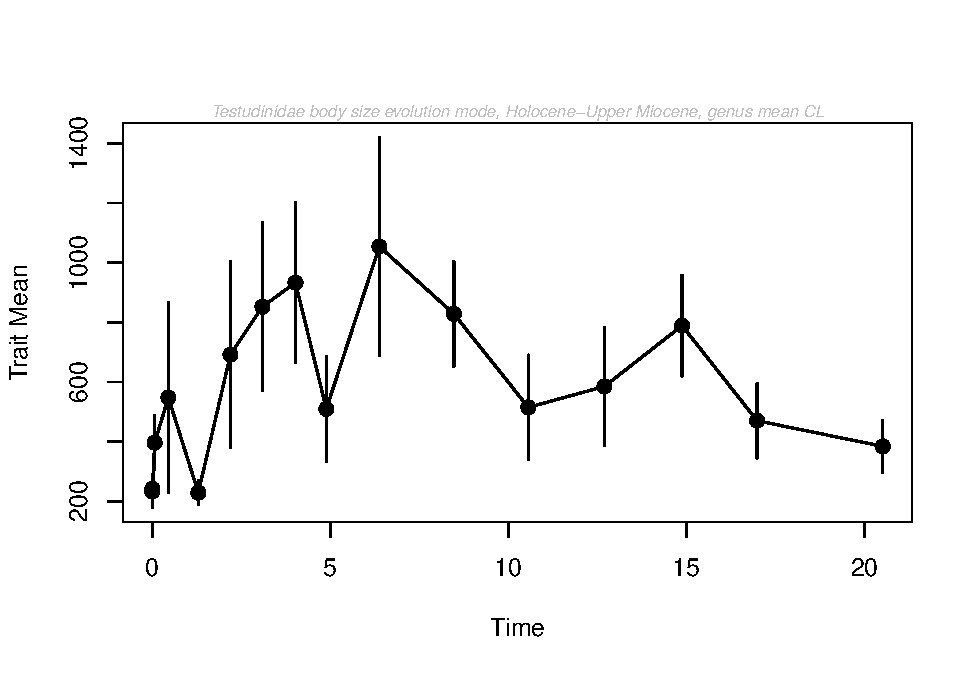
\includegraphics{MA_JJ_files/figure-latex/paleoTS plot with genus mean, excluding island species-1.pdf}
\caption{paleoTS plot with genus mean, excluding island species}
\end{figure}

\begin{longtable}[]{@{}lrrrr@{}}
\caption{Model-fitting results for testudinidae, genera, excluding
insular species}\tabularnewline
\toprule
& logL & K & AICc & Akaike.wt\tabularnewline
\midrule
\endfirsthead
\toprule
& logL & K & AICc & Akaike.wt\tabularnewline
\midrule
\endhead
GRW & -82.26287 & 2 & 169.8591 & 0.300\tabularnewline
URW & -83.12577 & 1 & 168.6515 & 0.548\tabularnewline
Stasis & -82.93984 & 2 & 171.2130 & 0.152\tabularnewline
\bottomrule
\end{longtable}

\newpage

\subsection{insular (excluding
continental)}\label{insular-excluding-continental}

\subsubsection{genera (insular)}\label{genera-insular}

\begin{figure}[htbp]
\centering
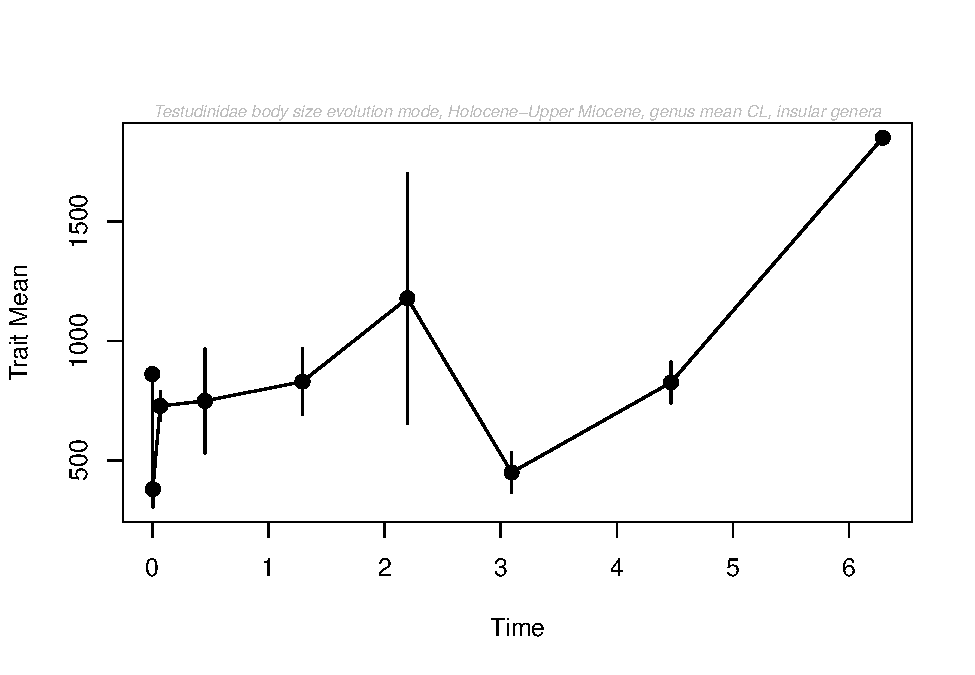
\includegraphics{MA_JJ_files/figure-latex/paleoTS plot with genus mean, excluding continental species-1.pdf}
\caption{paleoTS plot with genus mean, only insular species}
\end{figure}

\begin{longtable}[]{@{}lrrrr@{}}
\caption{Model-fitting results for testudinidae, genera, only insular
species}\tabularnewline
\toprule
& logL & K & AICc & Akaike.wt\tabularnewline
\midrule
\endfirsthead
\toprule
& logL & K & AICc & Akaike.wt\tabularnewline
\midrule
\endhead
GRW & -68.57344 & 2 & 143.5469 & 0\tabularnewline
URW & -75.76576 & 1 & 154.1982 & 0\tabularnewline
Stasis & -60.41581 & 2 & 127.2316 & 1\tabularnewline
\bottomrule
\end{longtable}

\newpage

\subsection{per continent}\label{per-continent}

\subsubsection{Europe, smaller original bins (see Table 2),
genera}\label{europe-smaller-original-bins-see-table-2-genera}

\begin{figure}[htbp]
\centering
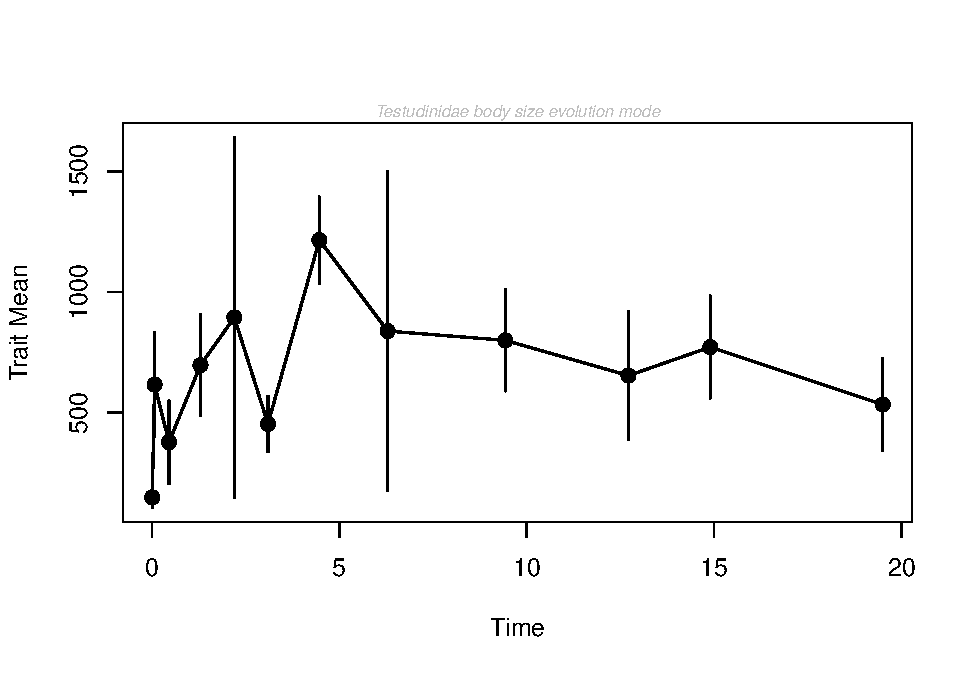
\includegraphics{MA_JJ_files/figure-latex/paleoTS with different time bins, no bins, genera, Europe-1.pdf}
\caption{Smaller original bins, genera, Europe}
\end{figure}

\begin{longtable}[]{@{}lrrrr@{}}
\caption{Model-fitting results for testudinidae, no bins,
genera}\tabularnewline
\toprule
& logL & K & AICc & Akaike.wt\tabularnewline
\midrule
\endfirsthead
\toprule
& logL & K & AICc & Akaike.wt\tabularnewline
\midrule
\endhead
GRW & -84.14010 & 2 & 173.7802 & 0.006\tabularnewline
URW & -85.90727 & 1 & 174.2590 & 0.005\tabularnewline
Stasis & -79.01365 & 2 & 163.5273 & 0.990\tabularnewline
\bottomrule
\end{longtable}

\newpage

\paragraph{Europe, smaller original bins (see Table 2), genera,
continental}\label{europe-smaller-original-bins-see-table-2-genera-continental}

\begin{figure}[htbp]
\centering
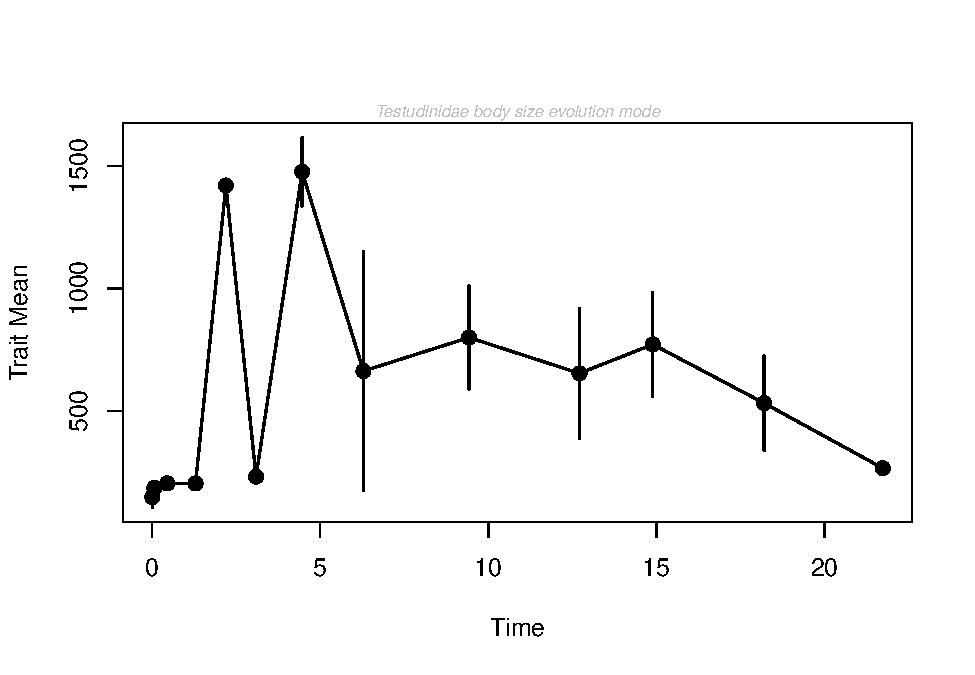
\includegraphics{MA_JJ_files/figure-latex/paleoTS with different time bins, no bins, genera, Europe, continental-1.pdf}
\caption{Smaller original bins, genera, Europe, continental}
\end{figure}

\begin{longtable}[]{@{}lrrrr@{}}
\caption{Model-fitting results for testudinidae, no bins,
genera}\tabularnewline
\toprule
& logL & K & AICc & Akaike.wt\tabularnewline
\midrule
\endfirsthead
\toprule
& logL & K & AICc & Akaike.wt\tabularnewline
\midrule
\endhead
GRW & -87.93137 & 2 & 181.3627 & 0.009\tabularnewline
URW & -92.56882 & 1 & 187.5821 & 0.000\tabularnewline
Stasis & -83.21073 & 2 & 171.9215 & 0.991\tabularnewline
\bottomrule
\end{longtable}

\newpage

\paragraph{Europe, smaller original bins (see Table 2), genera,
insular}\label{europe-smaller-original-bins-see-table-2-genera-insular}

\begin{figure}[htbp]
\centering
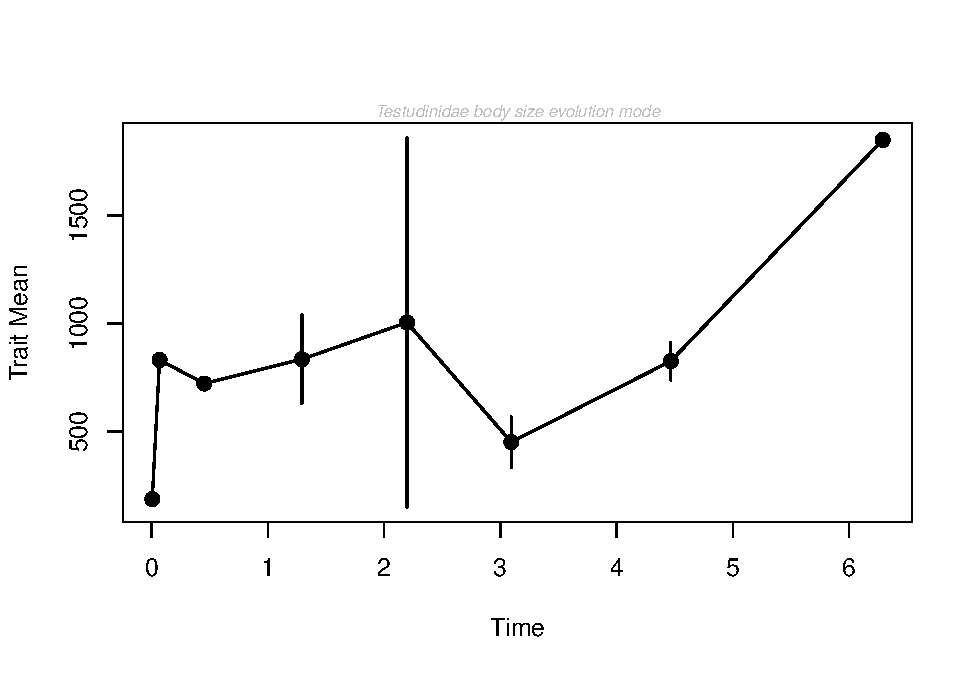
\includegraphics{MA_JJ_files/figure-latex/paleoTS with different time bins, no bins, genera, Europe, insular-1.pdf}
\caption{Smaller original bins, genera, Europe, insular}
\end{figure}

\begin{longtable}[]{@{}lrrrr@{}}
\caption{Model-fitting results for testudinidae, no bins,
genera}\tabularnewline
\toprule
& logL & K & AICc & Akaike.wt\tabularnewline
\midrule
\endfirsthead
\toprule
& logL & K & AICc & Akaike.wt\tabularnewline
\midrule
\endhead
GRW & -67.12192 & 2 & 141.2438 & 0.000\tabularnewline
URW & -57.51634 & 1 & 117.8327 & 0.074\tabularnewline
Stasis & -52.89638 & 2 & 112.7928 & 0.926\tabularnewline
\bottomrule
\end{longtable}

\newpage 

\subsubsection{Eurasia, smaller original bins (See Table 2),
genera}\label{eurasia-smaller-original-bins-see-table-2-genera}

\begin{figure}[htbp]
\centering
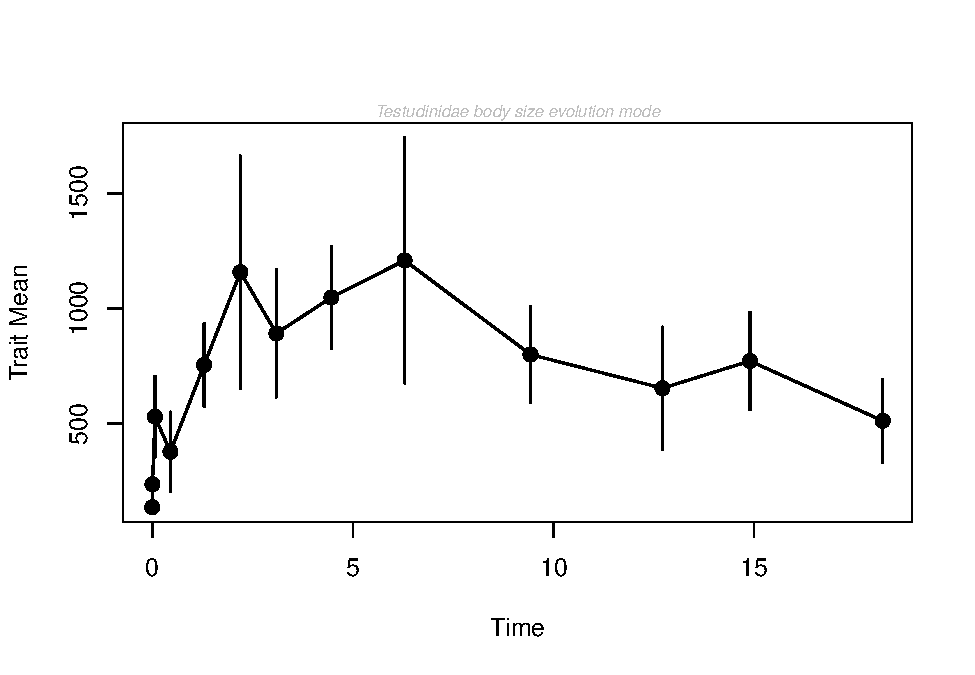
\includegraphics{MA_JJ_files/figure-latex/paleoTS with different time bins, no bins, genera, Eurasia-1.pdf}
\caption{Smaller original bins, genera, Eurasia}
\end{figure}

\begin{longtable}[]{@{}lrrrr@{}}
\caption{Model-fitting results for testudinidae, no bins,
genera}\tabularnewline
\toprule
& logL & K & AICc & Akaike.wt\tabularnewline
\midrule
\endfirsthead
\toprule
& logL & K & AICc & Akaike.wt\tabularnewline
\midrule
\endhead
GRW & -85.25195 & 2 & 175.8372 & 0.149\tabularnewline
URW & -85.39072 & 1 & 173.1814 & 0.562\tabularnewline
Stasis & -84.58890 & 2 & 174.5111 & 0.289\tabularnewline
\bottomrule
\end{longtable}

\newpage 

\subsubsection{Eurasia, smaller original bins (See Table 2), genera,
continental}\label{eurasia-smaller-original-bins-see-table-2-genera-continental}

\begin{figure}[htbp]
\centering
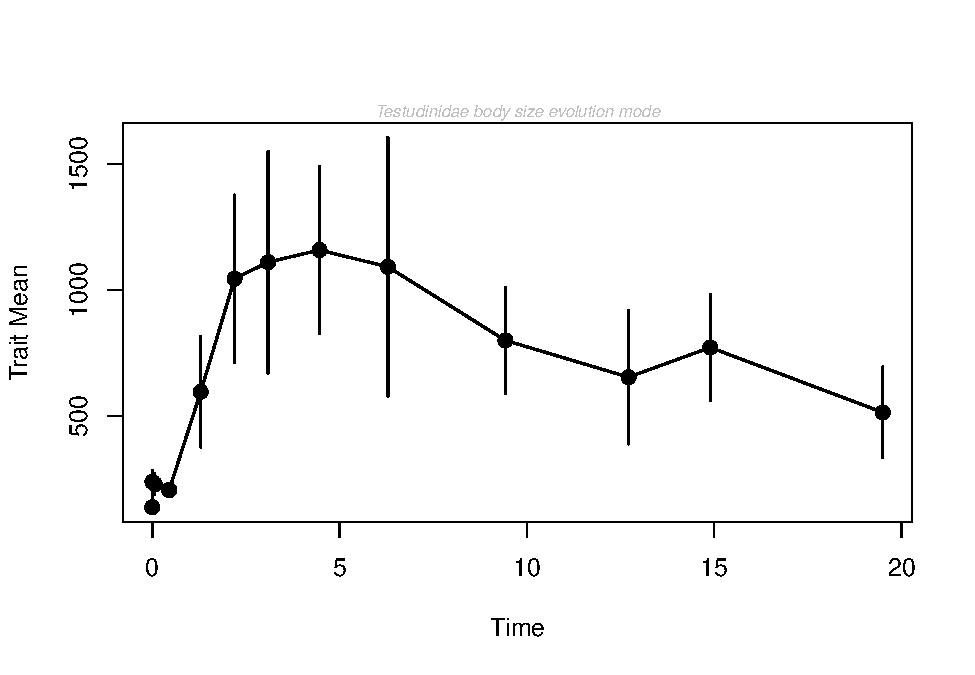
\includegraphics{MA_JJ_files/figure-latex/paleoTS with different time bins, no bins, genera, Eurasia, continental-1.pdf}
\caption{Smaller original bins, genera, Eurasia, continental}
\end{figure}

\begin{longtable}[]{@{}lrrrr@{}}
\caption{Model-fitting results for testudinidae, no bins,
genera}\tabularnewline
\toprule
& logL & K & AICc & Akaike.wt\tabularnewline
\midrule
\endfirsthead
\toprule
& logL & K & AICc & Akaike.wt\tabularnewline
\midrule
\endhead
GRW & -82.20698 & 2 & 169.7473 & 0.222\tabularnewline
URW & -82.42344 & 1 & 167.2469 & 0.776\tabularnewline
Stasis & -87.19538 & 2 & 179.7241 & 0.002\tabularnewline
\bottomrule
\end{longtable}

\newpage 

\subsubsection{Eurasia, smaller original bins (See Table 2), genera,
insular}\label{eurasia-smaller-original-bins-see-table-2-genera-insular}

\begin{figure}[htbp]
\centering
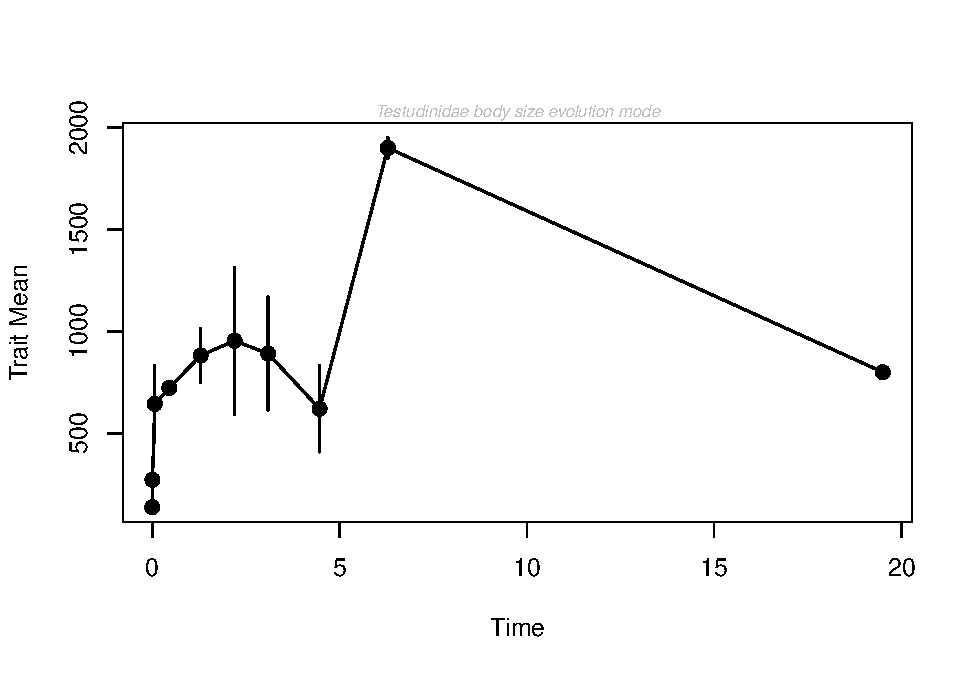
\includegraphics{MA_JJ_files/figure-latex/paleoTS with different time bins, no bins, genera, Eurasia, insular-1.pdf}
\caption{Smaller original bins, genera, Eurasia, insular}
\end{figure}

\begin{longtable}[]{@{}lrrrr@{}}
\caption{Model-fitting results for testudinidae, no bins,
genera}\tabularnewline
\toprule
& logL & K & AICc & Akaike.wt\tabularnewline
\midrule
\endfirsthead
\toprule
& logL & K & AICc & Akaike.wt\tabularnewline
\midrule
\endhead
GRW & -69.56419 & 2 & 145.1284 & 0.193\tabularnewline
URW & -71.67437 & 1 & 145.9202 & 0.130\tabularnewline
Stasis & -68.31026 & 2 & 142.6205 & 0.677\tabularnewline
\bottomrule
\end{longtable}


\end{document}
